\documentclass[a4paper,12pt]{article}

\usepackage[utf8]{inputenc}
\usepackage[T1]{fontenc}
\usepackage[polish]{babel}
\usepackage{polski}
\usepackage{geometry}
\geometry{top=2.5cm, bottom=2.5cm, left=2.5cm, right=2.5cm}

\usepackage{amsmath}
\usepackage{amssymb}
\usepackage{graphicx}
\usepackage{float}
\usepackage{booktabs}
\usepackage{color}
\usepackage{caption}
\usepackage{subcaption}
\usepackage[colorlinks=true, linkcolor=black, citecolor=black, urlcolor=blue]{hyperref}

% Konfiguracja formatowania kodu (R)
\usepackage{listings}
\definecolor{codegreen}{rgb}{0,0.6,0}
\definecolor{codegray}{rgb}{0.5,0.5,0.5}
\definecolor{codepurple}{rgb}{0.58,0,0.82}
\definecolor{backcolour}{rgb}{0.95,0.95,0.92}

\lstdefinestyle{Rstyle}{
    backgroundcolor=\color{backcolour},   
    commentstyle=\color{codegreen},
    keywordstyle=\color{blue},
    numberstyle=\tiny\color{codegray},
    stringstyle=\color{codepurple},
    basicstyle=\ttfamily\footnotesize,
    breakatwhitespace=false,         
    breaklines=true,                 
    captionpos=b,                    
    keepspaces=true,                 
    numbers=left,                    
    numbersep=5pt,                  
    showspaces=false,                
    showstringspaces=false,
    showtabs=false,                  
    tabsize=2,
    language=R
}
\lstset{style=Rstyle}

% ==============================================================================
% STRONA TYTUŁOWA
% ==============================================================================
\title{
    \vspace{-2cm}
    \begin{center}
        \Large \textbf{Politechnika Wrocławska} \\ % TODO: Wpisz swoją uczelnię
    \end{center}
    \vspace{2cm}
    \Large Inteligencja Obliczeniowa i jej zastosowania \\
    \vspace{0.5cm}
    \Huge \textbf{Sprawozdanie 1} \\
    \vspace{0.5cm}
    \Large Badanie algorytmów genetycznych na przykładzie optymalizacji wielomodalnych funkcji ciągłych
}
\author{
    \textbf{Autorzy:} Jakub Jaśków 268416, Justyna Ziemichód 268431 % TODO: Wpisz swoje dane
}
\date{\today}

\begin{document}

\maketitle
\thispagestyle{empty}

\newpage
\tableofcontents
\newpage

% ------------------------------------------------------------------------------
\section{Cel cwiczeń}
% ------------------------------------------------------------------------------
Celem laboratorium jest praktyczne zbadanie skuteczności algorytmów genetycznych (GA) w poszukiwaniu minimum globalnego dla wielomodalnych, nieliniowych funkcji ciągłych. Główny nacisk położono na empiryczną analizę wpływu kluczowych parametrów algorytmu (wielkośc populacji, liczba pokoleń, wpływ elityzmu) oraz obecności operatorów ewolucyjnych (krzyżowania i mutacji) na zbieżnośc i zdolność ucieczki z ekstremów lokalnych.

% ------------------------------------------------------------------------------
\section{Optymalizowane funkcje}
% ------------------------------------------------------------------------------
Badania przeprowadzono na dwóch dwuwymiarowych funkcjach ciągłych w dziedzinie $x_1, x_2 \in [-5.12, 5.12]$. 

\subsection{Funkcja Rastrigina}
Wzór funkcji przyjmuje postać \cite{muehlenbein1991}:
\begin{equation}
f(x_1, x_2) = 20 + \sum_{i=1}^{2} \left[ x_i^2 - 10\cos(2\pi x_i) \right]
\end{equation}
Jest to funkcja separowalna (zmienne można optymalizować niezależnie). Posiada rozległą, regularną siatkę minimów lokalnych. Optimum globalne wynosi $f(0,0) = 0$.

\begin{figure}[H]
    \centering
    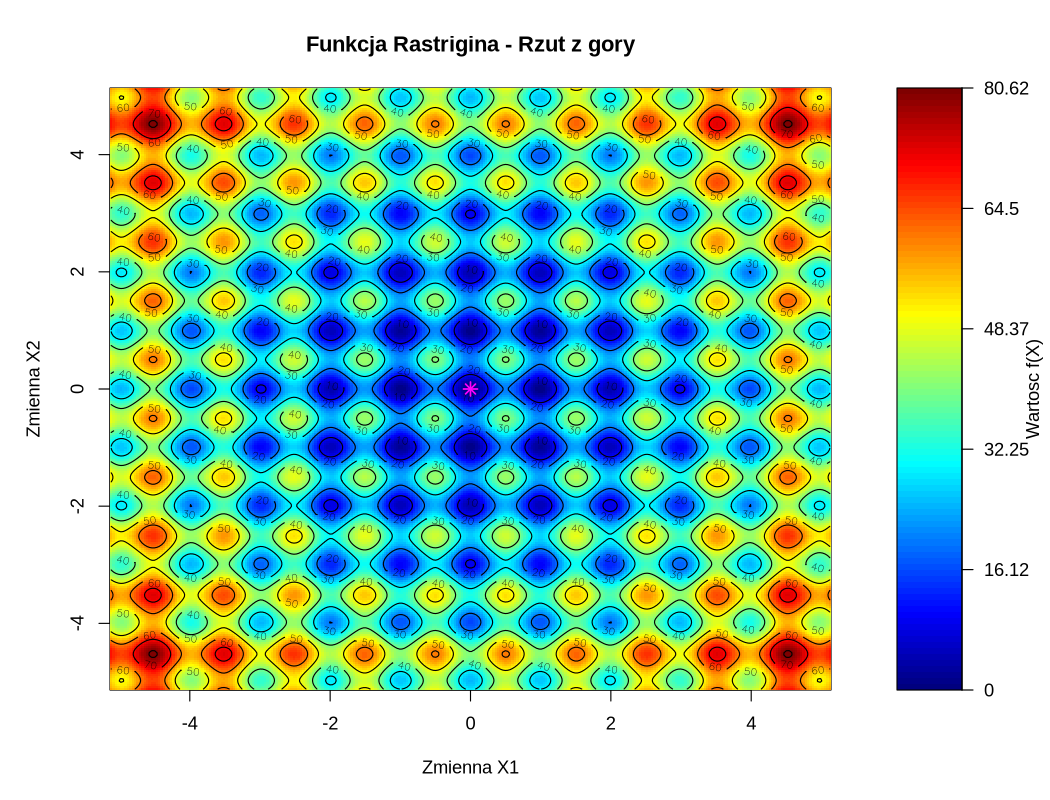
\includegraphics[width=0.48\textwidth]{img/1_rastrigin_rzut_gory.png}
    \hfill
    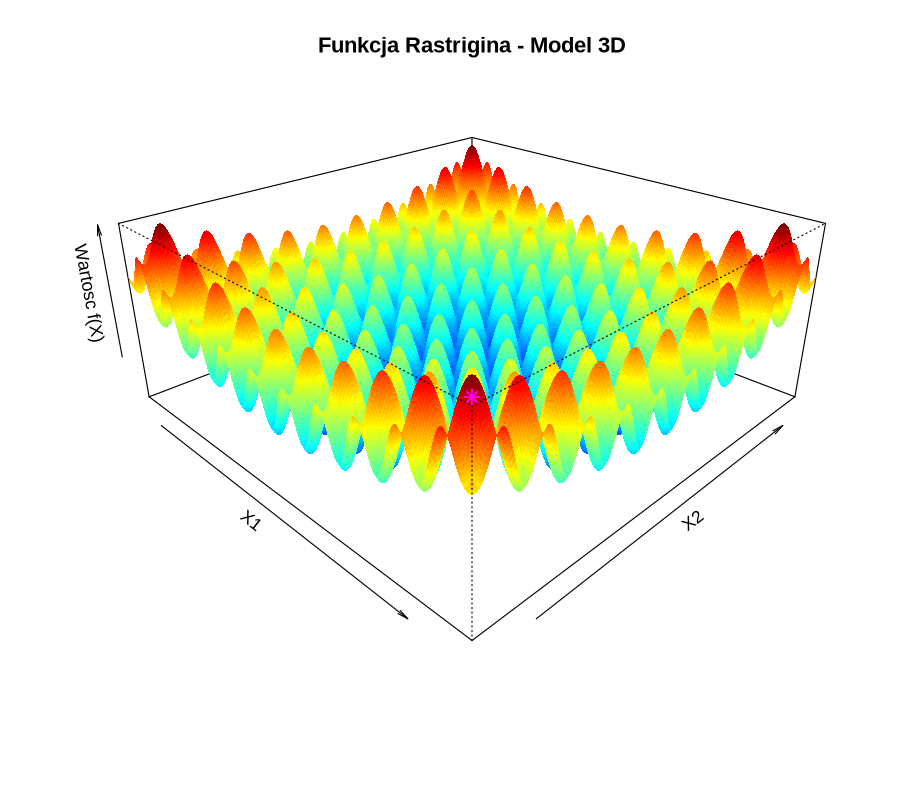
\includegraphics[width=0.48\textwidth]{img/2_rastrigin_model_3d.png}
    \caption{Funkcja Rastrigina: rzut z góry z warstwicami (po lewej) oraz model 3D (po prawej).}
    \label{fig:func_rastrigin}
\end{figure}

\subsection{Funkcja Schaffer nr 2}
Wzór funkcji określa równanie \cite{schaffer1989}:
\begin{equation}
f(x_1, x_2) = 0.5 + \frac{\sin^2\left(\sqrt{x_1^2 + x_2^2}\right) - 0.5}{\left[1 + 0.001\left(x_1^2 + x_2^2\right)\right]^2}
\end{equation}
Jest to funkcja nieseparowalna o silnej zależności i symetrii kołowej. Optimum globalne $f(0,0) = 0$ ukryte jest za stromymi, koncentrycznymi barierami potencjału.

\begin{figure}[H]
    \centering
    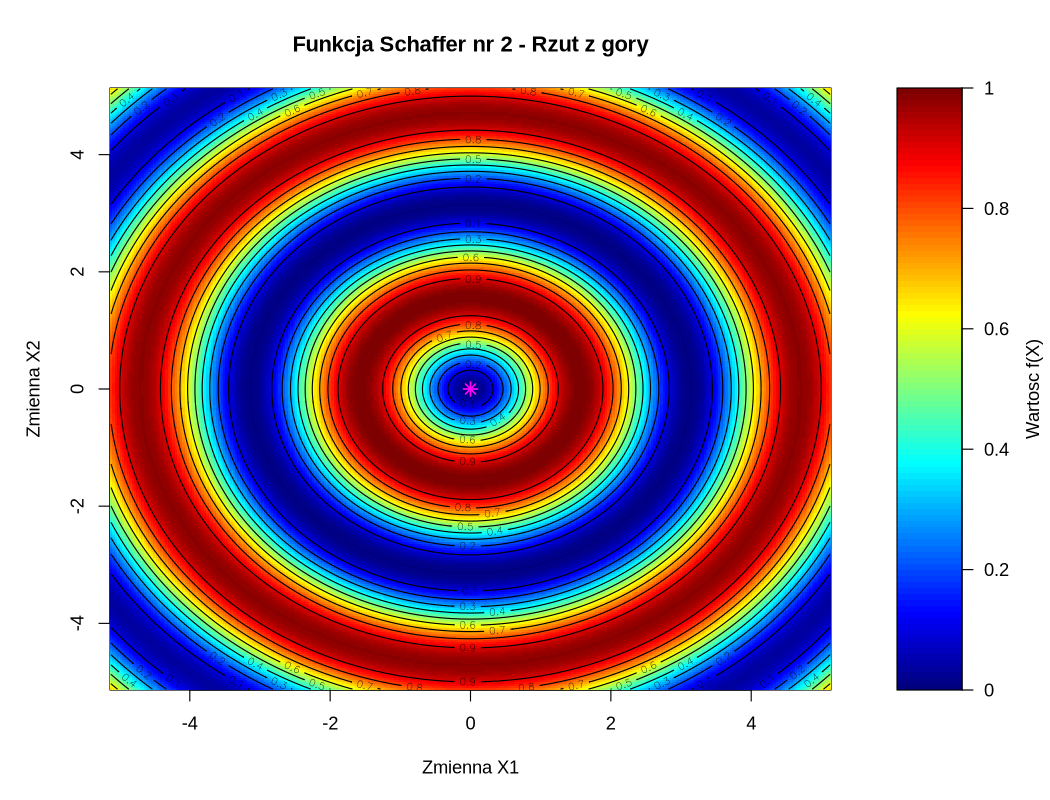
\includegraphics[width=0.48\textwidth]{img/3_schaffer_rzut_gory.png}
    \hfill
    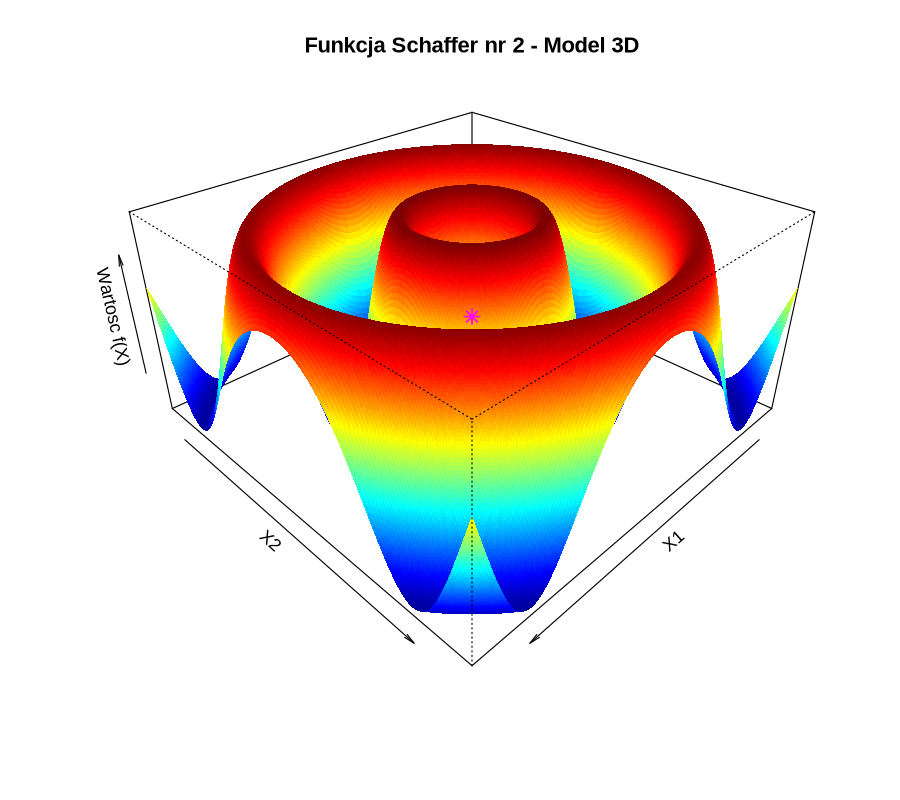
\includegraphics[width=0.48\textwidth]{img/4_schaffer_model_3d.png}
    \caption{Funkcja Schaffer nr 2: rzut z góry (po lewej) oraz model 3D (po prawej).}
    \label{fig:func_schaffer}
\end{figure}

% ------------------------------------------------------------------------------
\section{Zastosowany algorytm optymalizacji}
% ------------------------------------------------------------------------------
Zastosowano klasyczny Algorytm Genetyczny (GA) – heurystykę przeszukiwania opartą na mechanizmach ewolucji naturalnej \cite{michalewicz1996, goldberg1995}. Algorytm operuje na populacji osobników reprezentujących potencjalne rozwiązania. Ocena ich jakości następuje poprzez funkcję przystosowania (fitness). Do reprodukcji wybierane są najlepsze jednostki (selekcja proporcjonalna/ruletkowa). Generowanie nowych rozwiązań realizowane jest poprzez operator krzyżowania (wymiana cech między rodzicami – odpowiada za eksploatację) oraz mutację (losowe zaburzenia – odpowiada za eksplorację). Zastosowano również elityzm, aby zagwarantować bezwarunkowe przetrwanie najlepszym osobnikom.

% ------------------------------------------------------------------------------
\section{Narzędzia implementacji i biblioteki}
% ------------------------------------------------------------------------------
Skrypt badawczy zaimplementowano w środowisku obliczeniowym \textbf{R} \cite{r-manual}. Głównym silnikiem optymalizacyjnym była biblioteka \texttt{GA} \cite{scrucca2013}. Zastosowano następujące podejście implementacyjne:
\begin{itemize}
    \item \textbf{Reprezentacja genów:} Ze względu na ciągły charakter badanych funkcji, wybrano kodowanie rzeczywisto-liczbowe (\texttt{type = "real-valued"}). Chromosom stanowił wektor $(x_1, x_2)$.
    \item \textbf{Przystosowanie do minimalizacji:} Biblioteka \texttt{GA} domyślnie przeprowadza maksymalizację. Aby rozwiązać problem poszukiwania minimum, zaimplementowano matematyczną transformację polegającą na negacji funkcji celu: $Fitness(x) = -f(x)$.
\end{itemize}


% ------------------------------------------------------------------------------
\section{Wybrane wartości i estymatory statystyczne}
% ------------------------------------------------------------------------------
Z uwagi na probabilistyczny (stochastyczny) charakter operatorów algorytmu genetycznego (losowa inicjalizacja populacji, ruletkowa selekcja, losowość krzyżowania i mutacji), pojedyncze wywołanie algorytmu nie jest miarodajne. Istnieje ryzyko uzyskania wyniku zaburzonego przez przypadek (np. przedwczesna zbieżność wywołana niefortunną populacją początkową).

Aby zagwarantować obiektywność i powtarzalność wyników, \textbf{każda unikalna konfiguracja parametrów była uruchamiana niezależnie 10-krotnie} ($N=10$). 


\subsection{Badane parametry}

W celu dokładnego zbadania trendów, parametry poddano ewaluacji na równomiernej siatce wartości. Dla wielkości populacji, liczby pokoleń oraz elityzmu zastosowano po 8 punktów pomiarowych, natomiast dla prawdopodobieństwa mutacji i krzyżowania po 20 punktów pomiarowych:

\begin{itemize}
    \item \textbf{Wielkość populacji (\texttt{popSize}):} $\{20, 40, 60, 80, 100, 120, 140, 160\}$
    \item \textbf{Liczba pokoleń (\texttt{maxiter}):} $\{20, 40, 60, 80, 100, 120, 140, 160\}$
    \item \textbf{Rozmiar elityzmu (\texttt{elitism}):} $\{0, 2, 4, 6, 8, 10, 12, 14\}$
    \item \textbf{Prawdopodobieństwo mutacji (\texttt{pmutation}):} 20 równomiernie rozmieszczonych wartości z przedziału $[0, 1]$
    \item \textbf{Prawdopodobieństwo krzyżowania (\texttt{pcrossover}):} 20 równomiernie rozmieszczonych wartości z przedziału $[0, 1]$
\end{itemize}

Jako konfigurację bazową przyjęto populację liczącą 40 osobników, 40 pokoleń, elityzm równy 2, prawdopodobieństwo mutacji wynoszące $0{,}1$ oraz prawdopodobieństwo krzyżowania wynoszące $0{,}8$. Następnie dla każdego analizowanego parametru wykonywano serię eksperymentów obejmującą różne wartości badanego ustawienia, przy zachowaniu pozostałych parametrów na poziomie bazowym.

Dodatkowo przeprowadzono eksperyment zależności krzyżowej pomiędzy prawdopodobieństwem mutacji i prawdopodobieństwem krzyżowania. W tym celu utworzono siatkę $20 \times 20$, obejmującą wszystkie kombinacje wartości $p_m$ i $p_c$ z przedziału $[0, 1]$. Wyniki przedstawiono w formie map ciepła, które pozwalają ocenić nie tylko osobny wpływ każdego operatora, lecz także ich łączne oddziaływanie na jakość znajdowanych rozwiązań.

W ostatnim etapie zbadano przebieg ewolucji przy wyłączonych operatorach genetycznych. Przeanalizowano trzy scenariusze: brak mutacji ($p_m = 0$), brak krzyżowania ($p_c = 0$) oraz jednoczesny brak mutacji i krzyżowania, co odpowiada sytuacji, w której działa wyłącznie mechanizm selekcji. Eksperyment ten pozwolił określić znaczenie poszczególnych operatorów w procesie poszukiwania rozwiązań.

Ze względu na losowy charakter algorytmu genetycznego każdy eksperyment powtórzono dziesięciokrotnie. Jako wynik przyjmowano średnią wartość najlepszego znalezionego rozwiązania uzyskaną we wszystkich uruchomieniach. Takie podejście pozwala ograniczyć wpływ przypadkowych odchyleń i uzyskać bardziej reprezentatywną ocenę skuteczności poszczególnych konfiguracji.

\subsection{Budowa estymatora błędu}
Jako główną miarę skuteczności algorytmu przyjęto estymator wartości oczekiwanej błędu końcowego. Obliczono go jako średnią arytmetyczną z bezwzględnych odchyleń znalezionego minimum od znanego, analitycznego minimum globalnego funkcji ($f(x^*) = 0$):
\begin{equation}
    \hat{\mu} = \frac{1}{N} \sum_{i=1}^{N} |f(x_{opt_i}) - f(x^*)| = \frac{1}{10} \sum_{i=1}^{10} |f(x_{opt_i})|
\end{equation}
Wartość ta reprezentuje oczekiwaną odległość (w wymiarze funkcji celu $Z$), w jakiej zatrzyma się algorytm od idealnego rozwiązania. Im wartość estymatora $\hat{\mu}$ jest bliższa zeru, tym wyższa skuteczność danej konfiguracji GA.



\subsection{Ewolucja i wizualizacja dynamiki chmary punktów}

Poniższe wykresy obrazują dynamikę przemieszczania się populacji (białe punkty) w przestrzeni poszukiwań na przestrzeni wybranych generacji. Pozwala to zaobserwować płynne przejście algorytmu od fazy globalnej eksploracji do lokalnej eksploatacji wokół znalezionych minimów.

\subsubsection*{Analiza zbieżności na funkcji Rastrigina} 

\begin{figure}[H]
    \centering
    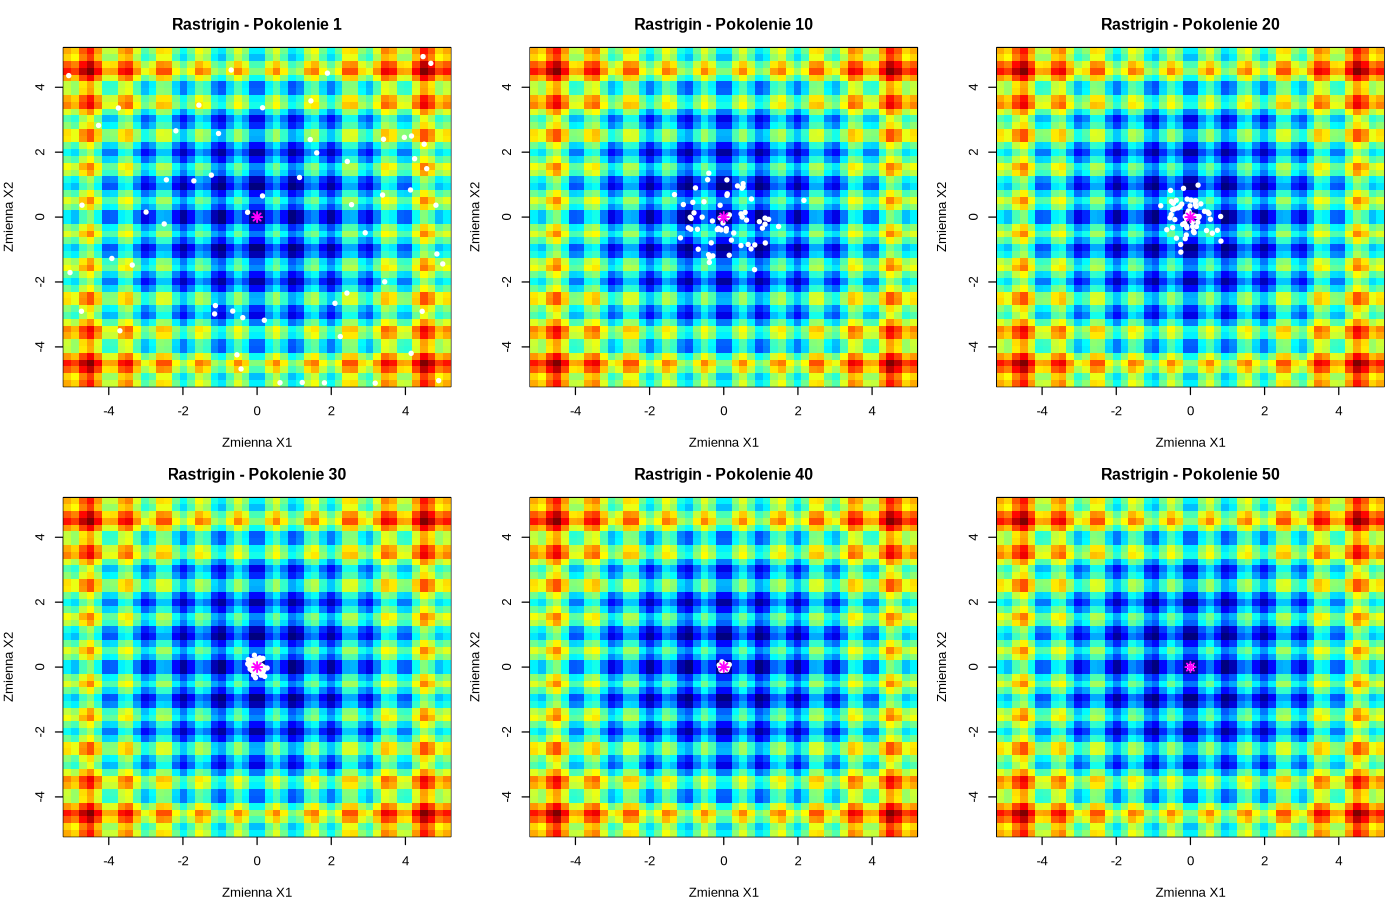
\includegraphics[width=\textwidth]{img/5_rastrigin_ewolucja_populacji.png}
    \caption{Dynamika ewolucji populacji dla funkcji Rastrigina w pokoleniach: 1, 10, 20, 30, 40 i 50.}
    \label{fig:ewolucja_rastrigin}
\end{figure}

W pierwszym pokoleniu populacja jest rozproszona równomiernie w całej dziedzinie (faza silnej eksploracji). Już w 10. generacji widoczna jest wyraźna tendencja do grupowania się osobników w zagłębieniach minimów lokalnych. Wraz z upływem czasu (pokolenia 20--30) algorytm skutecznie odrzuca gorsze zapadnie, kierując osobniki w stronę centrum układu współrzędnych. Pomiędzy 40. a 50. pokoleniem następuje niemal całkowita zbieżność -- chmara punktów gęsto koncentruje się dokładnie na optimum globalnym. Świadczy to o bardzo dobrej radzeniu sobie standardowego GA z separowalnymi funkcjami wielomodalnymi.

\subsubsection*{Analiza zbieżności na funkcji Schaffer nr 2} 

\begin{figure}[H]
    \centering
    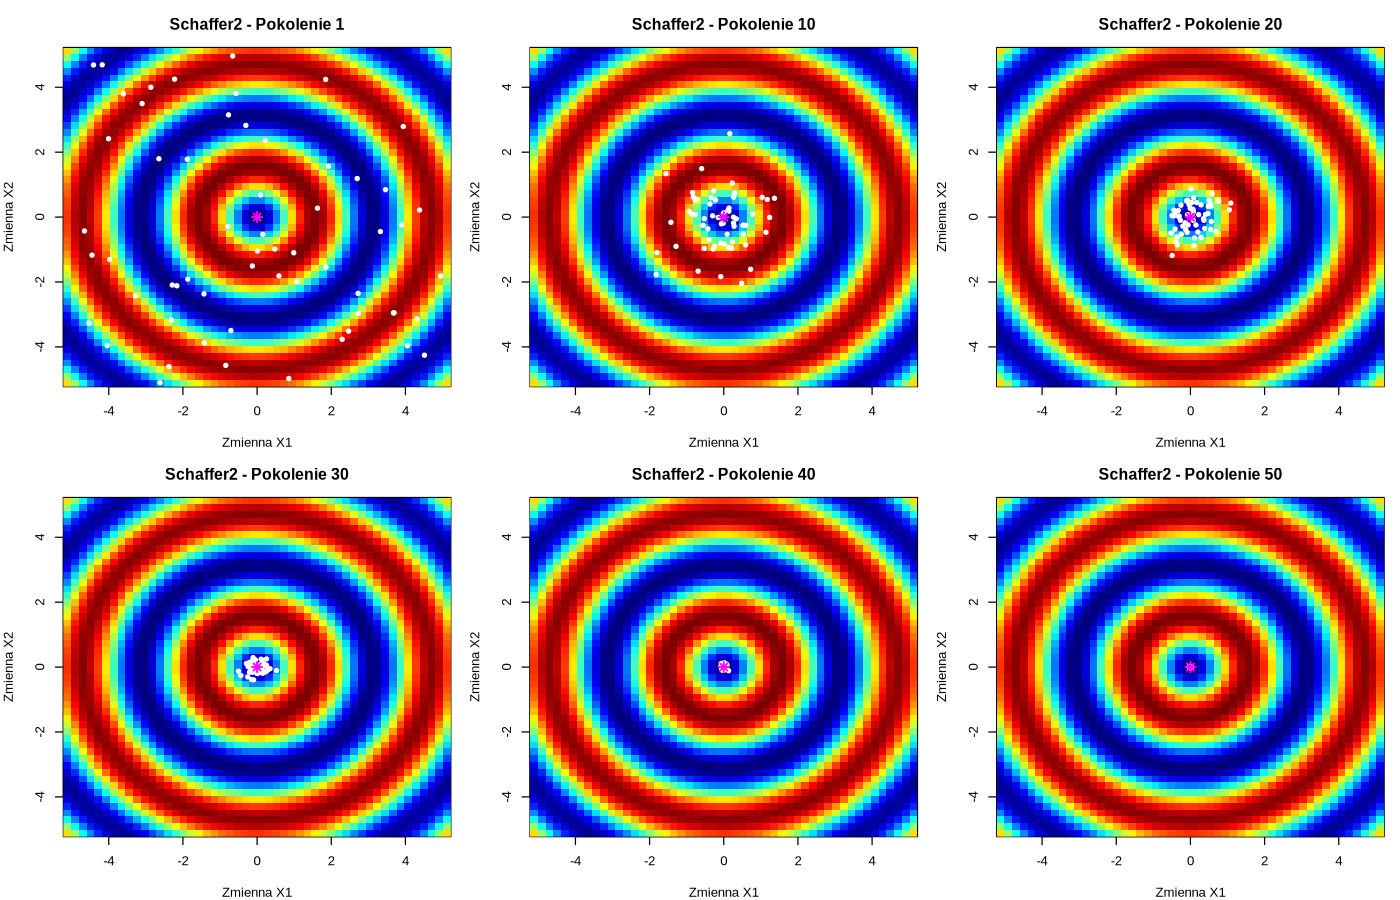
\includegraphics[width=\textwidth]{img/6_schaffer_ewolucja_populacji.png}
    \caption{Dynamika ewolucji populacji dla funkcji Schaffer nr 2 w pokoleniach: 1, 10, 20, 30, 40 i 50.}
    \label{fig:ewolucja_schaffer}
\end{figure}

Początkowy rozkład jest analogiczny jak w poprzednim przypadku. Algorytm dość szybko (około 10. pokolenia) odnajduje centralny, najbardziej stromy obszar funkcji. Zauważalna jest jednak fundamentalna różnica -- chmara punktów osiada w głębokim, koncentrycznym minimum lokalnym (pierścieniu) bezpośrednio otaczającym optimum globalne. Od 20. aż do 50. pokolenia większość populacji pozostaje „uwięziona” w tej strefie. Bariera potencjału między owym pierścieniem a centralnym, absolutnym minimum jest na tyle stroma, że pojedyncze osobniki z trudem przeskakują do właściwego optimum.

\subsection{Wpływ poszczególnych parametrów na wyniki}

W tej sekcji zbadano izolowany wpływ pięciu kluczowych parametrów algorytmu na zdolność minimalizacji błędu: wielkości populacji, liczby pokoleń, rozmiaru elityzmu oraz prawdopodobieństwa mutacji i krzyżowania. Analiza opiera się na rzetelnym estymatorze błędu uśrednionym z 10 niezależnych przebiegów.

\subsubsection*{Funkcja Rastrigina}

% --- Populacja Rastrigin ---
\begin{figure}[H]
    \centering
    \begin{minipage}[c]{0.3\textwidth}
        \centering
        \small
        \begin{tabular}{cc}
        \toprule
        \textbf{Pop.} & \textbf{Błąd ($\hat{\mu}$)} \\
        \midrule
        20 & 0.330800 \\
        40 & 0.012068 \\
        60 & 0.012447 \\
        80 & 0.000905 \\
        100 & 0.000251 \\
        120 & 0.005087 \\
        140 & 0.002445 \\
        160 & 0.000840 \\
        \bottomrule
        \end{tabular}
    \end{minipage}\hfill
    \begin{minipage}[c]{0.65\textwidth}
        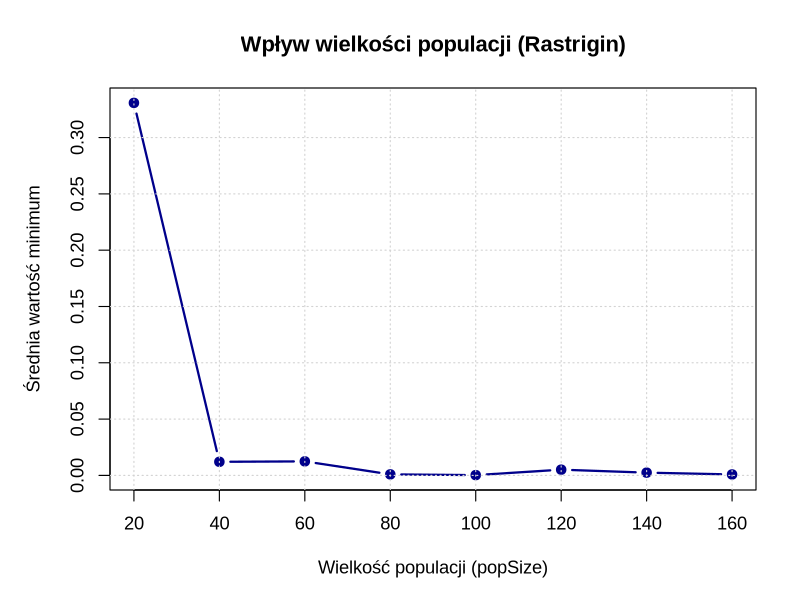
\includegraphics[width=\textwidth]{img/7a_rastrigin_wplyw_populacji.png}
    \end{minipage}
    \caption{Wpływ wielkości populacji na średni błąd dla funkcji Rastrigina.}
    \label{fig:rastrigin_pop}
\end{figure}

\textbf{Populacja (Wykres \ref{fig:rastrigin_pop}):} Zwiększenie liczby osobników z 20 do 40 powoduje gwałtowny spadek błędu z około 0.33 do 0.01. Dalszy wzrost populacji przynosi już znacznie mniejsze korzyści, choć najlepsze wyniki uzyskano dla populacji liczącej 100 osobników. Wyniki sugerują, że dla funkcji Rastrigina kluczowe jest zapewnienie odpowiedniej różnorodności genetycznej populacji. Zbyt mała liczba osobników utrudnia skuteczne przeszukiwanie silnie wielomodalnej przestrzeni rozwiązań i zwiększa ryzyko przedwczesnej zbieżności do minimów lokalnych.

% --- Pokolenia Rastrigin ---
\begin{figure}[H]
    \centering
    \begin{minipage}[c]{0.3\textwidth}
        \centering
        \small
        \begin{tabular}{cc}
        \toprule
        \textbf{Iter.} & \textbf{Błąd ($\hat{\mu}$)} \\
        \midrule
        20 & 0.038918 \\
        40 & 0.053924 \\
        60 & 0.001108 \\
        80 & 0.001045 \\
        100 & 0.000086 \\
        120 & 0.000402 \\
        140 & 0.000003 \\
        160 & 0.000005 \\
        \bottomrule
        \end{tabular}
    \end{minipage}\hfill
    \begin{minipage}[c]{0.65\textwidth}
        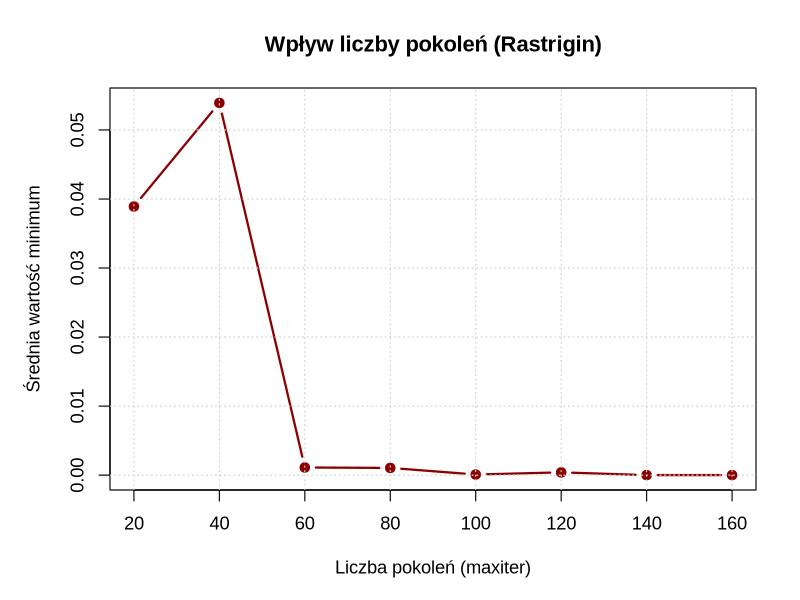
\includegraphics[width=\textwidth]{img/7b_rastrigin_wplyw_pokolen.png}
    \end{minipage}
    \caption{Wpływ liczby pokoleń na średni błąd dla funkcji Rastrigina.}
    \label{fig:rastrigin_iter}
\end{figure}

\textbf{Pokolenia (Wykres \ref{fig:rastrigin_iter}):} Wraz ze wzrostem liczby pokoleń obserwowany jest wyraźny spadek błędu. Szczególnie istotna poprawa następuje pomiędzy 40 a 60 pokoleniem, gdzie błąd maleje o niemal dwa rzędy wielkości. Dalsze zwiększanie liczby iteracji nadal poprawia wyniki, jednak korzyści stają się coraz mniejsze. Oznacza to, że algorytm potrzebuje odpowiednio długiego procesu ewolucji do skutecznego opuszczania minimów lokalnych i stopniowego zbliżania się do optimum globalnego.

% --- Elityzm Rastrigin ---
\begin{figure}[H]
    \centering
    \begin{minipage}[c]{0.3\textwidth}
        \centering
        \small
        \begin{tabular}{cc}
        \toprule
        \textbf{Elita} & \textbf{Błąd ($\hat{\mu}$)} \\
        \midrule
        0 & 0.928872 \\
        2 & 0.011724 \\
        4 & 0.016856 \\
        6 & 0.121797 \\
        8 & 0.180057 \\
        10 & 0.003769 \\
        12 & 0.092451 \\
        14 & 0.203502 \\
        \bottomrule
        \end{tabular}
    \end{minipage}\hfill
    \begin{minipage}[c]{0.65\textwidth}
        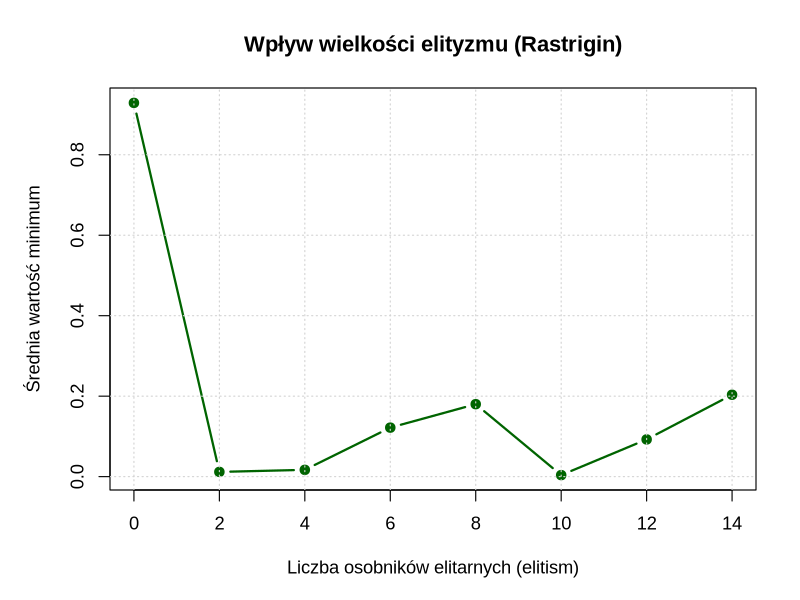
\includegraphics[width=\textwidth]{img/7c_rastrigin_wplyw_elityzmu.png}
    \end{minipage}
    \caption{Wpływ elityzmu na średni błąd dla funkcji Rastrigina.}
    \label{fig:rastrigin_elit}
\end{figure}

\textbf{Elityzm (Wykres \ref{fig:rastrigin_elit}):} Brak elityzmu prowadzi do bardzo wysokiego błędu (0.93), co wskazuje na częstą utratę najlepszych rozwiązań wskutek działania operatorów genetycznych. Już niewielka elita znacząco poprawia skuteczność algorytmu. Jednocześnie zależność nie ma charakteru monotonicznego. Dla części wartości elityzmu (6, 8, 12 oraz 14) następuje wyraźne pogorszenie wyników, natomiast dla wartości 10 uzyskano jeden z najlepszych rezultatów. Sugeruje to, że wpływ elityzmu jest silnie zależny od równowagi pomiędzy ochroną najlepszych osobników a utrzymaniem różnorodności populacji. Zbyt mała elita zwiększa ryzyko utraty dobrych rozwiązań, natomiast zbyt duża może prowadzić do stagnacji i ograniczenia eksploracji przestrzeni poszukiwań.

% --- Mutacja Rastrigin ---
\begin{figure}[H]
    \centering
    \begin{minipage}[c]{0.3\textwidth}
        \centering
        \footnotesize
        \begin{tabular}{cc}
        \toprule
        \textbf{Mut.} & \textbf{Błąd ($\hat{\mu}$)} \\
        \midrule
        1.00 & 0.785825 \\
        0.89 & 0.727237 \\
        0.79 & 0.666263 \\
        0.68 & 0.497069 \\
        0.58 & 0.452899 \\
        0.47 & 0.112850 \\
        0.37 & 0.021628 \\
        0.26 & 0.009737 \\
        0.16 & 0.013538 \\
        0.05 & 0.155117 \\
        0.00 & 0.549088 \\
        \bottomrule
        \end{tabular}
    \end{minipage}\hfill
    \begin{minipage}[c]{0.65\textwidth}
        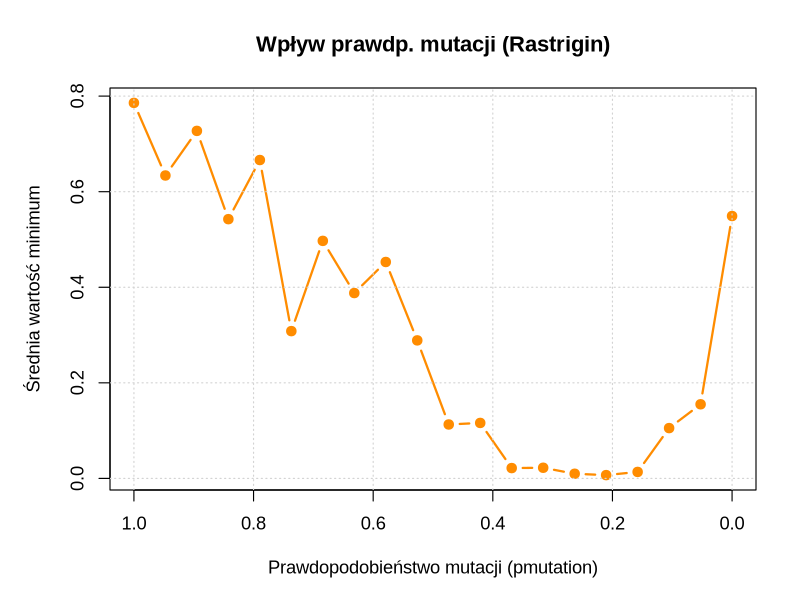
\includegraphics[width=\textwidth]{img/9a_rastrigin_wplyw_mutacji.png}
    \end{minipage}
    \caption{Wpływ prawdopodobieństwa mutacji dla funkcji Rastrigina.}
    \label{fig:rastrigin_mut}
\end{figure}

\textbf{Mutacja (Wykres \ref{fig:rastrigin_mut}):} Zarówno brak mutacji, jak i bardzo wysokie prawdopodobieństwo mutacji prowadzą do pogorszenia jakości rozwiązań. Przy $p_m = 0$ błąd osiąga wartość około 0.55, co wskazuje na przedwczesną zbieżność populacji i utratę zdolności eksploracji nowych obszarów przestrzeni rozwiązań. Z kolei wysokie wartości mutacji ($p_m > 0.5$) powodują dominację losowych zmian nad procesem selekcji, przez co algorytm zaczyna przypominać przeszukiwanie losowe. Najlepsze wyniki uzyskano dla umiarkowanych wartości mutacji, około $p_m \in [0.15, 0.30]$. Oznacza to, że funkcja Rastrigina wymaga zachowania równowagi pomiędzy eksploracją nowych rozwiązań a eksploatacją już odnalezionych obiecujących regionów.

% --- Krzyzowanie Rastrigin ---
\begin{figure}[H]
    \centering
    \begin{minipage}[c]{0.3\textwidth}
        \centering
        \footnotesize
        \begin{tabular}{cc}
        \toprule
        \textbf{Krzyż.} & \textbf{Błąd ($\hat{\mu}$)} \\
        \midrule
        1.00 & 0.004252 \\
        0.89 & 0.168955 \\
        0.79 & 0.201764 \\
        0.68 & 0.154828 \\
        0.58 & 0.127000 \\
        0.47 & 0.123248 \\
        0.37 & 0.407881 \\
        0.26 & 0.455852 \\
        0.16 & 0.436457 \\
        0.05 & 1.206640 \\
        0.00 & 1.492429 \\
        \bottomrule
        \end{tabular}
    \end{minipage}\hfill
    \begin{minipage}[c]{0.65\textwidth}
        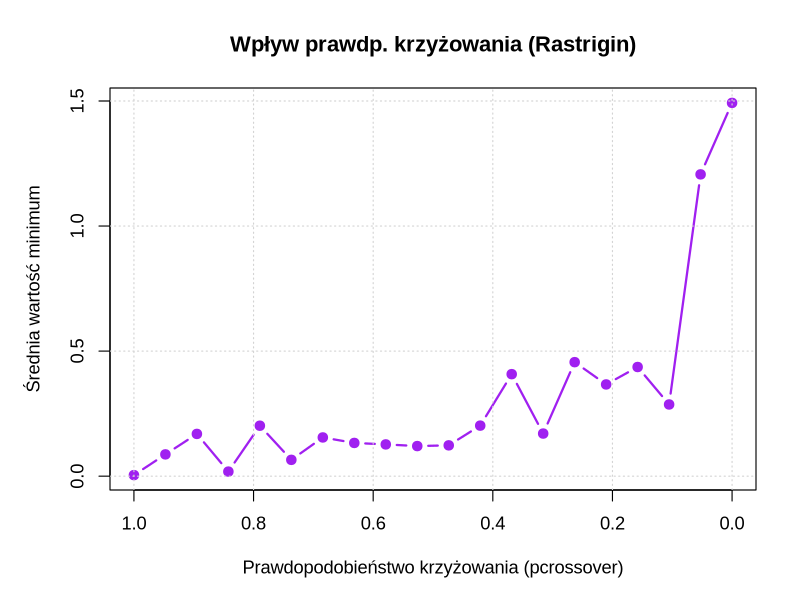
\includegraphics[width=\textwidth]{img/9b_rastrigin_wplyw_krzyzowania.png}
    \end{minipage}
    \caption{Wpływ prawdopodobieństwa krzyżowania dla funkcji Rastrigina.}
    \label{fig:rastrigin_krzyz}
\end{figure}

\textbf{Krzyżowanie (Wykres \ref{fig:rastrigin_krzyz}):} Spośród analizowanych parametrów prawdopodobieństwo krzyżowania wywiera jeden z najsilniejszych wpływów na skuteczność algorytmu. Wraz ze wzrostem $p_c$ błąd wyraźnie maleje. Najlepszy wynik uzyskano dla $p_c = 1.0$, gdzie błąd wyniósł około $0.004$, natomiast brak krzyżowania zwiększał błąd do około $1.49$. Wskazuje to, że dla funkcji Rastrigina rekombinacja materiału genetycznego jest kluczowym mechanizmem poprawy wyników.

Znaczenie krzyżowania można powiązać ze strukturą funkcji Rastrigina. Jest to funkcja silnie wielomodalna, ale jednocześnie separowalna, co oznacza, że poszczególne zmienne mogą być optymalizowane względnie niezależnie. Dzięki temu krzyżowanie może skutecznie łączyć korzystne wartości różnych współrzędnych pochodzące od różnych osobników. Rekombinacja przyspiesza więc budowanie lepszych rozwiązań, ponieważ algorytm nie musi odnajdywać całego rozwiązania w jednym osobniku.

Aby uzupełnić analizę pojedynczego wpływu krzyżowania, zbadano również zależność krzyżową między prawdopodobieństwem mutacji i krzyżowania. Wyniki przedstawiono na mapie ciepła na rysunku~\ref{fig:rastrigin_heatmap}.

\begin{figure}[H]
    \centering
    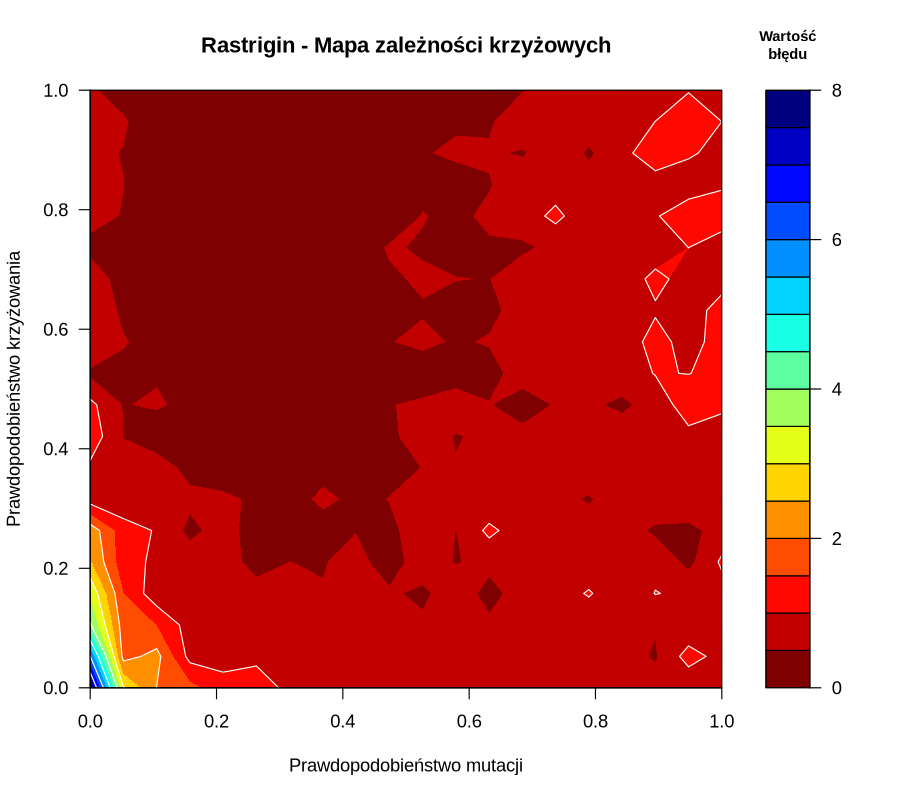
\includegraphics[width=0.8\textwidth]{img/11_rastrigin_mapa_ciepla.png}
    \caption{Mapa ciepła dla funkcji Rastrigina. Czerwony kolor oznacza mniejszy błąd (lepsze rozwiązanie).}
    \label{fig:rastrigin_heatmap}
\end{figure}

Mapa ciepła potwierdza, że najwyższy błąd pojawia się przy jednocześnie bardzo małych wartościach mutacji i krzyżowania. W takiej konfiguracji algorytm traci podstawowe źródła zmienności, przez co populacja łatwo zatrzymuje się w minimach lokalnych. Jest to szczególnie istotne dla funkcji Rastrigina, której krajobraz zawiera wiele minimów lokalnych.

Najkorzystniejszy obszar znajduje się głównie przy wysokim $p_c$ oraz niskim lub umiarkowanym $p_m$. Oznacza to, że w badanej konfiguracji największe znaczenie miała rekombinacja informacji między osobnikami, natomiast mutacja pełniła funkcję równoważącą. Jej umiarkowany poziom wspierał utrzymanie różnorodności i umożliwiał opuszczanie słabszych minimów lokalnych, ale zbyt wysoka mutacja mogła nadmiernie zaburzać dobre rozwiązania.

Analiza parametrów oraz ich zależności krzyżowej prowadzi do wniosku, że funkcja Rastrigina wymaga jednocześnie wysokiej różnorodności populacji i intensywnej wymiany informacji między osobnikami. Największe znaczenie mają wysokie prawdopodobieństwo krzyżowania, umiarkowana mutacja oraz obecność elityzmu zabezpieczającego przed utratą najlepszych rozwiązań.

\subsubsection*{Funkcja Schaffer nr 2}

% --- Populacja Schaffer ---
\begin{figure}[H]
    \centering
    \begin{minipage}[c]{0.3\textwidth}
        \centering
        \small
        \begin{tabular}{cc}
        \toprule
        \textbf{Pop.} & \textbf{Błąd ($\hat{\mu}$)} \\
        \midrule
        20 & 0.008836 \\
        40 & 0.006822 \\
        60 & 0.005555 \\
        80 & 0.006354 \\
        100 & 0.006200 \\
        120 & 0.005301 \\
        140 & 0.001191 \\
        160 & 0.005504 \\
        \bottomrule
        \end{tabular}
    \end{minipage}\hfill
    \begin{minipage}[c]{0.65\textwidth}
        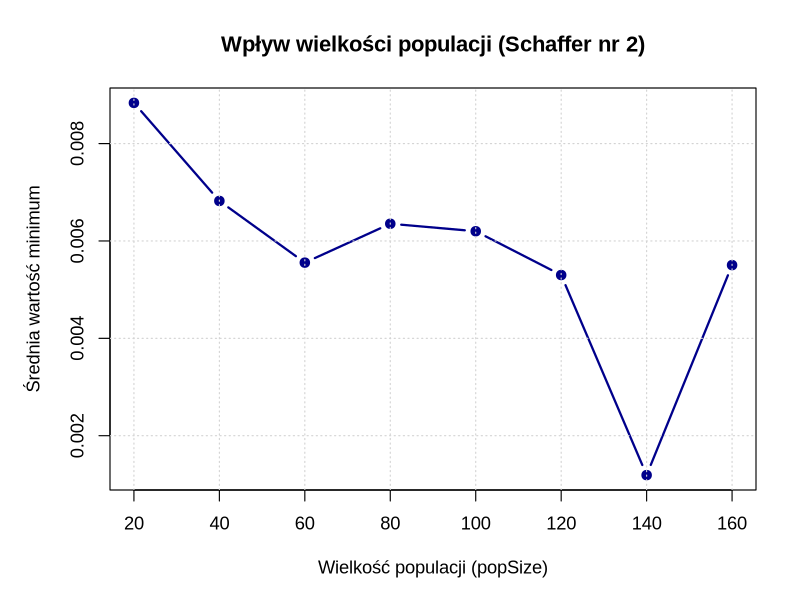
\includegraphics[width=\textwidth]{img/8a_schaffer_wplyw_populacji.png}
    \end{minipage}
    \caption{Wpływ wielkości populacji na średni błąd dla funkcji Schaffer nr 2.}
    \label{fig:schaffer_pop}
\end{figure}

\textbf{Populacja (Wykres \ref{fig:schaffer_pop}):} Zwiększanie liczebności populacji nie prowadzi do jednoznacznego, monotonicznego spadku błędu. Dla większości analizowanych wartości błąd utrzymuje się w wąskim przedziale od około $0{,}005$ do $0{,}009$. Najlepszy wynik uzyskano dla populacji liczącej 140 osobników, gdzie błąd spadł do około $0{,}001$, jednak ponowny wzrost błędu dla 160 osobników wskazuje, że nie można traktować tego punktu jako potwierdzenia stałego trendu. Wyniki sugerują, że w przypadku funkcji Schaffer nr 2 sama większa populacja nie gwarantuje poprawy jakości rozwiązania, a wpływ liczebności populacji jest słabszy niż dla funkcji Rastrigina.

% --- Pokolenia Schaffer ---
\begin{figure}[H]
    \centering
    \begin{minipage}[c]{0.3\textwidth}
        \centering
        \small
        \begin{tabular}{cc}
        \toprule
        \textbf{Iter.} & \textbf{Błąd ($\hat{\mu}$)} \\
        \midrule
        20 & 0.008902 \\
        40 & 0.006743 \\
        60 & 0.008920 \\
        80 & 0.004959 \\
        100 & 0.005979 \\
        120 & 0.008747 \\
        140 & 0.005451 \\
        160 & 0.005801 \\
        \bottomrule
        \end{tabular}
    \end{minipage}\hfill
    \begin{minipage}[c]{0.65\textwidth}
        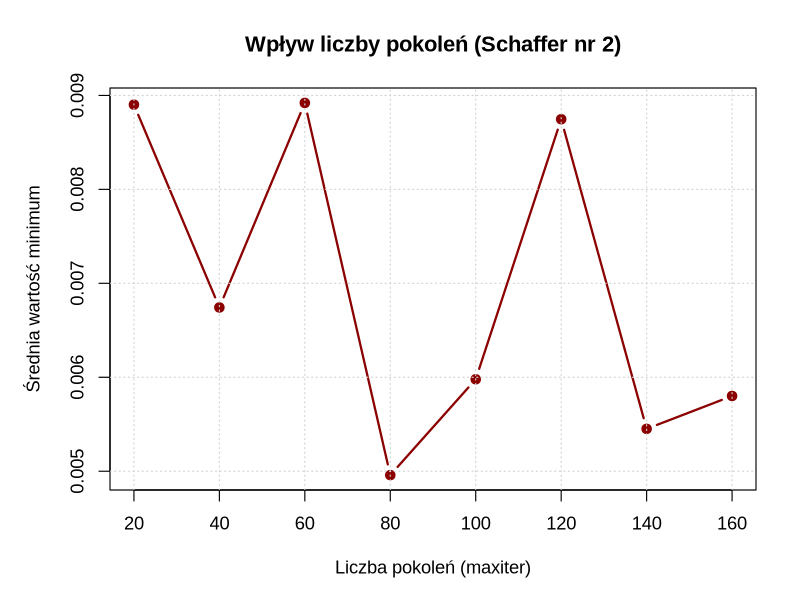
\includegraphics[width=\textwidth]{img/8b_schaffer_wplyw_pokolen.png}
    \end{minipage}
    \caption{Wpływ liczby pokoleń na średni błąd dla funkcji Schaffer nr 2.}
    \label{fig:schaffer_iter}
\end{figure}

\textbf{Pokolenia (Wykres \ref{fig:schaffer_iter}):} Zwiększanie liczby pokoleń również nie daje jednoznacznej poprawy wyników. Błąd oscyluje w zbliżonym zakresie, a najlepszy rezultat uzyskano dla 80 pokoleń, nie zaś dla największej liczby iteracji. Oznacza to, że wydłużenie procesu ewolucji nie przekłada się w tym przypadku bezpośrednio na lepszą zbieżność. Można przypuszczać, że algorytm stosunkowo szybko osiąga poziom rozwiązań charakterystyczny dla danej konfiguracji, a dalsze iteracje prowadzą głównie do wahań wynikających z losowego charakteru operatorów genetycznych.

% --- Elityzm Schaffer ---
\begin{figure}[H]
    \centering
    \begin{minipage}[c]{0.3\textwidth}
        \centering
        \small
        \begin{tabular}{cc}
        \toprule
        \textbf{Elita} & \textbf{Błąd ($\hat{\mu}$)} \\
        \midrule
        0 & 0.014423 \\
        2 & 0.007178 \\
        4 & 0.008195 \\
        6 & 0.006320 \\
        8 & 0.007773 \\
        10 & 0.008436 \\
        12 & 0.007994 \\
        14 & 0.006888 \\
        \bottomrule
        \end{tabular}
    \end{minipage}\hfill
    \begin{minipage}[c]{0.65\textwidth}
        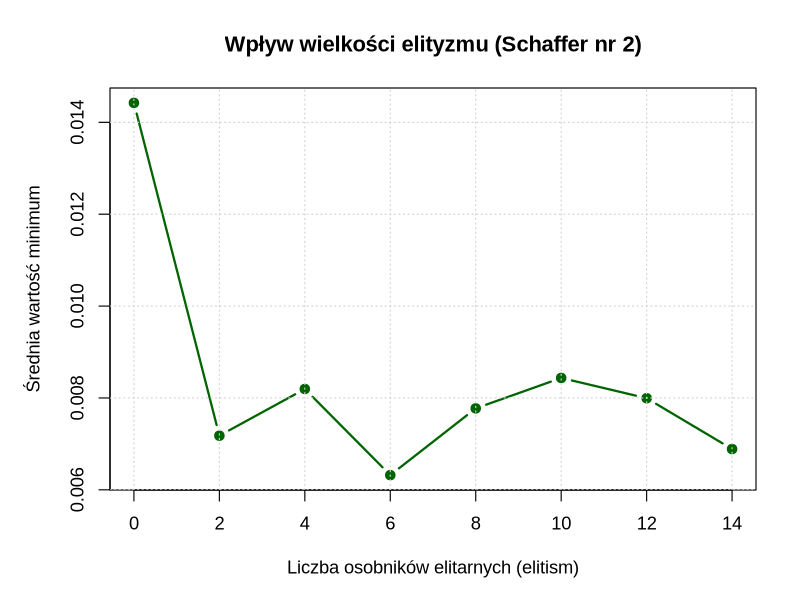
\includegraphics[width=\textwidth]{img/8c_schaffer_wplyw_elityzmu.png}
    \end{minipage}
    \caption{Wpływ elityzmu na średni błąd dla funkcji Schaffer nr 2.}
    \label{fig:schaffer_elit}
\end{figure}

\textbf{Elityzm (Wykres \ref{fig:schaffer_elit}):} Brak elityzmu prowadzi do najwyższego błędu spośród analizowanych wariantów, co wskazuje, że zachowanie najlepszych osobników jest korzystne również dla funkcji Schaffer nr 2. Po wprowadzeniu elity błąd spada mniej więcej do zakresu $0{,}006$--$0{,}008$, jednak dalsze zwiększanie liczby osobników elitarnych nie daje wyraźnego trendu poprawy. Najlepszy wynik uzyskano dla elity równej 6, ale wyniki dla pozostałych dodatnich wartości są do siebie zbliżone. Oznacza to, że elityzm pełni głównie funkcję stabilizującą, lecz jego dokładna wartość ma ograniczone znaczenie po przekroczeniu minimalnego poziomu ochrony najlepszych rozwiązań.

% --- Mutacja Schaffer ---
\begin{figure}[H]
    \centering
    \begin{minipage}[c]{0.3\textwidth}
        \centering
        \footnotesize
        \begin{tabular}{cc}
        \toprule
        \textbf{Mut.} & \textbf{Błąd ($\hat{\mu}$)} \\
        \midrule
        1.00 & 0.007927 \\
        0.89 & 0.005216 \\
        0.79 & 0.007440 \\
        0.68 & 0.004816 \\
        0.58 & 0.008484 \\
        0.47 & 0.005603 \\
        0.37 & 0.001992 \\
        0.26 & 0.005121 \\
        0.16 & 0.007318 \\
        0.05 & 0.007451 \\
        0.00 & 0.008744 \\
        \bottomrule
        \end{tabular}
    \end{minipage}\hfill
    \begin{minipage}[c]{0.65\textwidth}
        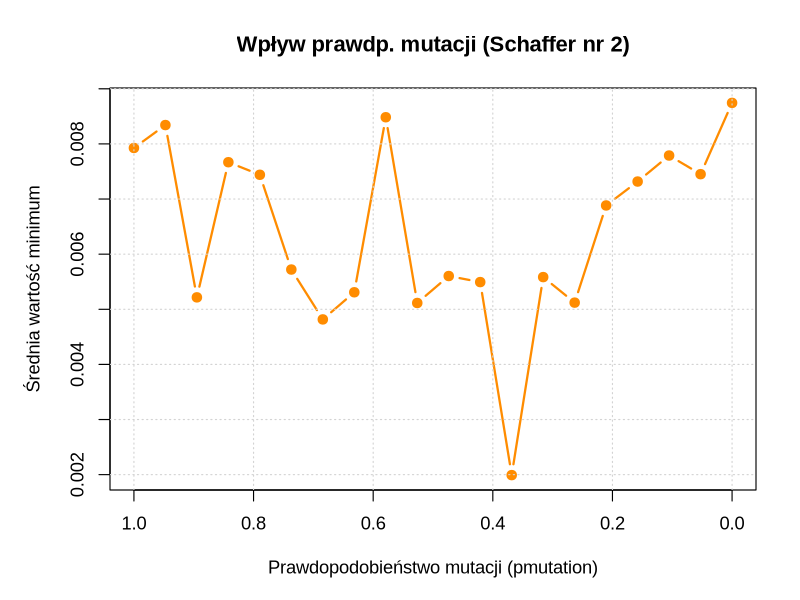
\includegraphics[width=\textwidth]{img/10a_schaffer_wplyw_mutacji.png}
    \end{minipage}
    \caption{Wpływ prawdopodobieństwa mutacji dla funkcji Schaffer nr 2.}
    \label{fig:schaffer_mut}
\end{figure}

\textbf{Mutacja (Wykres \ref{fig:schaffer_mut}):} Wpływ prawdopodobieństwa mutacji jest niemonotoniczny i znacznie słabszy niż w przypadku funkcji Rastrigina. Błąd dla większości wartości $p_m$ pozostaje na poziomie kilku tysięcznych. Najlepszy wynik uzyskano dla $p_m = 0{,}37$, jednak pojedynczy punkt minimum nie oznacza jednoznacznego globalnego trendu. Brak mutacji daje jeden z gorszych wyników, co wskazuje, że pewien poziom zmienności populacji jest potrzebny, ale bardzo wysokie wartości mutacji nie prowadzą do tak gwałtownego pogorszenia jak dla funkcji Rastrigina. Można więc uznać, że funkcja Schaffer nr 2 jest mniej wrażliwa na dobór prawdopodobieństwa mutacji.

% --- Krzyzowanie Schaffer ---
\begin{figure}[H]
    \centering
    \begin{minipage}[c]{0.3\textwidth}
        \centering
        \footnotesize
        \begin{tabular}{cc}
        \toprule
        \textbf{Krzyż.} & \textbf{Błąd ($\hat{\mu}$)} \\
        \midrule
        1.00 & 0.007364 \\
        0.89 & 0.008750 \\
        0.79 & 0.008543 \\
        0.68 & 0.006803 \\
        0.58 & 0.008746 \\
        0.47 & 0.006711 \\
        0.37 & 0.006266 \\
        0.26 & 0.009721 \\
        0.16 & 0.008924 \\
        0.05 & 0.008275 \\
        0.00 & 0.009959 \\
        \bottomrule
        \end{tabular}
    \end{minipage}\hfill
    \begin{minipage}[c]{0.65\textwidth}
        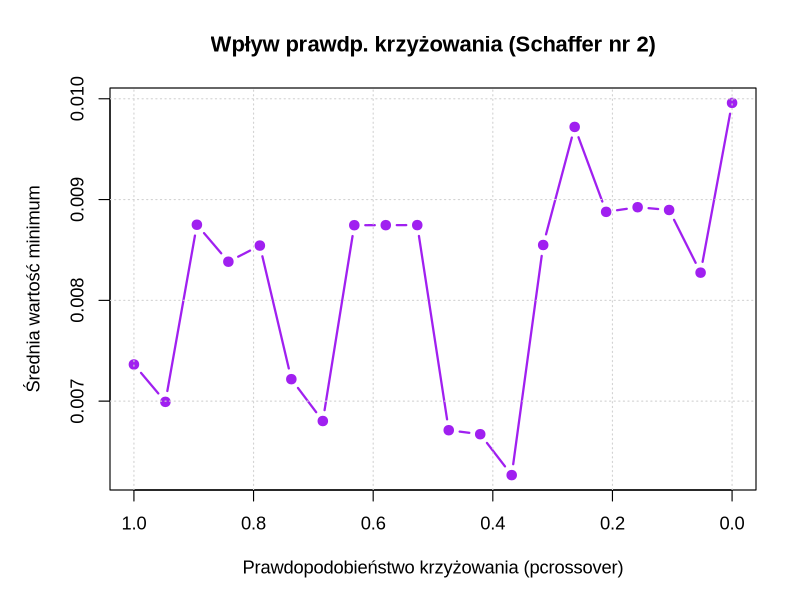
\includegraphics[width=\textwidth]{img/10b_schaffer_wplyw_krzyzowania.png}
    \end{minipage}
    \caption{Wpływ prawdopodobieństwa krzyżowania dla funkcji Schaffer nr 2.}
    \label{fig:schaffer_krzyz}
\end{figure}

\textbf{Krzyżowanie (Wykres \ref{fig:schaffer_krzyz}):} Zmiana prawdopodobieństwa krzyżowania nie powoduje dużych różnic w wartości błędu. Dla wszystkich analizowanych wartości $p_c$ wynik pozostaje w wąskim zakresie około $0{,}006$--$0{,}010$, a najniższy błąd uzyskano dla $p_c = 0{,}37$. Nie widać jednak trendu monotonicznego, co sugeruje, że krzyżowanie nie było głównym mechanizmem poprawy rozwiązań dla tej funkcji.

Można to wiązać z charakterem funkcji Schaffer nr 2, w której proste łączenie fragmentów osobników nie zawsze musi zachowywać korzystne relacje między zmiennymi. W przeciwieństwie do funkcji Rastrigina nie obserwuje się tutaj wyraźnej poprawy wraz ze wzrostem prawdopodobieństwa krzyżowania. Rekombinacja działa więc raczej jako operator pomocniczy niż dominujący mechanizm optymalizacji.

Aby uzupełnić analizę pojedynczego wpływu krzyżowania, zbadano również zależność krzyżową między prawdopodobieństwem mutacji i krzyżowania. Wyniki przedstawiono na mapie ciepła na rysunku~\ref{fig:schaffer_heatmap}.

\begin{figure}[H]
    \centering
    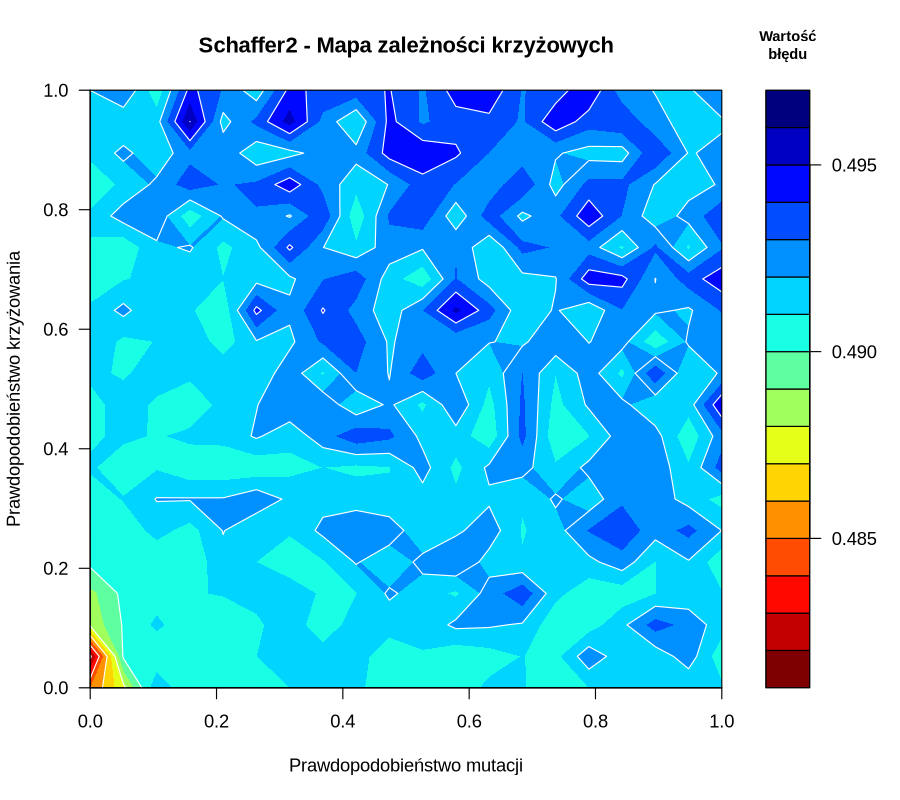
\includegraphics[width=0.8\textwidth]{img/12_schaffer_mapa_ciepla.png}
    \caption{Mapa ciepła dla funkcji Schaffer nr 2. Czerwony kolor oznacza mniejszy błąd (lepsze rozwiązanie).}
    \label{fig:schaffer_heatmap}
\end{figure}

Mapa ciepła potwierdza ograniczoną wrażliwość funkcji Schaffer nr 2 na dobór $p_m$ i $p_c$. Najniższy błąd występuje przy bardzo małych wartościach obu parametrów, co wskazuje, że w tej konfiguracji nadmierna eksploracja nie była potrzebna. W pozostałej części wykresu różnice są niewielkie, a skala błędu pozostaje wąska.

Widoczne przejście kolorów po przekątnej można interpretować jako efekt stopniowego wzrostu losowości procesu wraz ze zwiększaniem łącznej intensywności mutacji i krzyżowania. Mutacja mogła wspierać lokalne korekty i utrzymanie różnorodności, jednak jej natężenie, podobnie jak natężenie krzyżowania, nie decydowało jednoznacznie o jakości końcowego wyniku.

Analiza parametrów oraz ich zależności krzyżowej prowadzi do wniosku, że dla funkcji Schaffer nr 2 badany algorytm jest relatywnie mało wrażliwy na zmiany ustawień. Zwiększanie populacji, liczby pokoleń, mutacji lub krzyżowania nie prowadzi do systematycznej poprawy, lecz raczej do niewielkich wahań. Wystarczające okazuje się zachowanie podstawowej różnorodności populacji oraz minimalnej ochrony najlepszych osobników. W porównaniu z funkcją Rastrigina wpływ operatorów genetycznych jest więc wyraźnie słabszy, co potwierdza, że dobór parametrów powinien wynikać ze struktury konkretnej funkcji celu.

\subsection{Przebieg ewolucji przy wyłączonych operatorach}

Dodatkowo przeanalizowano przebieg ewolucji populacji po wyłączeniu wybranych operatorów genetycznych. Rozważono trzy warianty: brak mutacji ($p_m = 0$), brak krzyżowania ($p_c = 0$) oraz jednoczesny brak mutacji i krzyżowania, czyli sytuację, w której działa wyłącznie selekcja.

\begin{figure}[H]
    \centering
    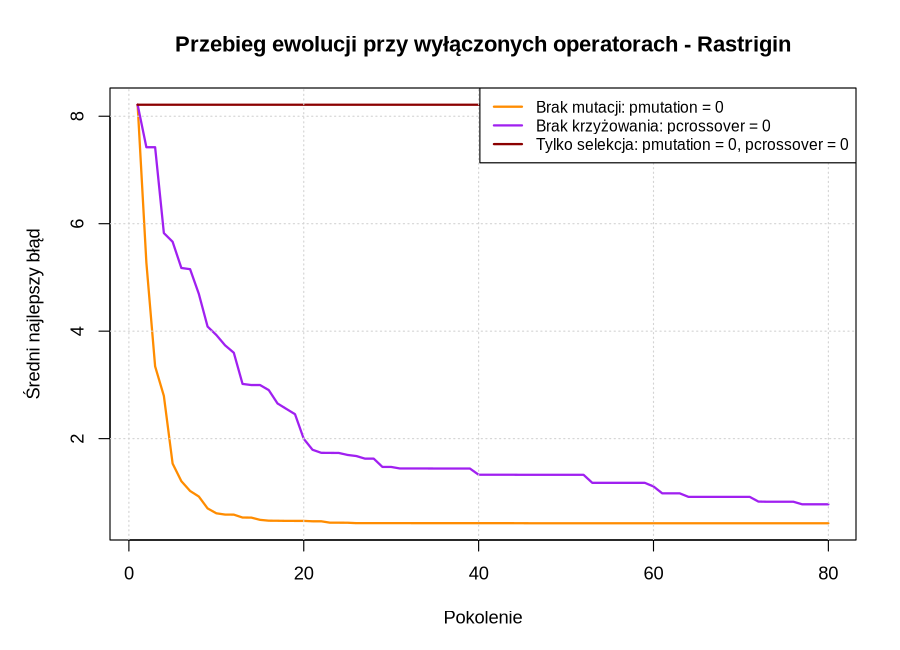
\includegraphics[width=0.8\textwidth]{img/15_rastrigin_ewolucja_wylaczone_operatory.png}
    \caption{Przebieg ewolucji dla funkcji Rastrigina przy wyłączonych operatorach genetycznych.}
    \label{fig:rastrigin_disabled_ops}
\end{figure}

\begin{figure}[H]
    \centering
    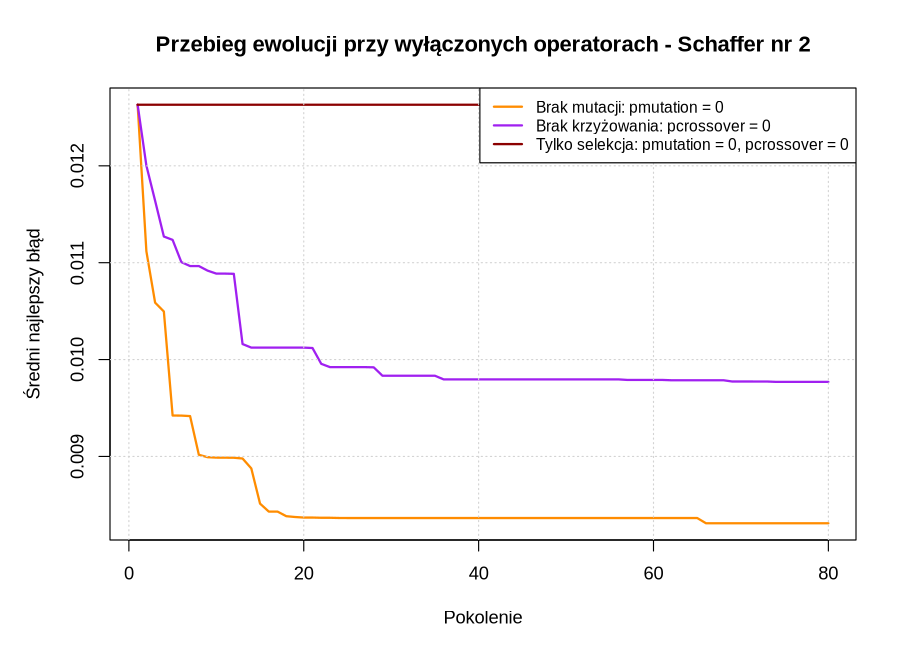
\includegraphics[width=0.8\textwidth]{img/16_schaffer_ewolucja_wylaczone_operatory.png}
    \caption{Przebieg ewolucji dla funkcji Schaffer nr 2 przy wyłączonych operatorach genetycznych.}
    \label{fig:schaffer_disabled_ops}
\end{figure}

\subsubsection*{Jak przebiega ewolucja przy wyłączonej mutacji?}

W obu analizowanych funkcjach populacja nadal była zdolna do poprawiania jakości rozwiązań pomimo wyłączenia mutacji. Oznacza to, że sam mechanizm krzyżowania połączony z selekcją był wystarczający do generowania coraz lepszych osobników. Szczególnie dobrze widoczne jest to dla funkcji Rastrigina, gdzie błąd szybko maleje już w początkowych pokoleniach.

Nie oznacza to jednak, że populacja zawsze równie łatwo znajduje rozwiązanie. Brak mutacji powoduje, że algorytm nie może generować nowych wartości genów, a jedynie rekombinować informacje obecne w populacji początkowej. Skuteczność zależy więc od tego, czy wśród początkowych osobników znajdują się odpowiednio dobre fragmenty rozwiązania, które mogą zostać połączone przez operator krzyżowania.

\subsubsection*{Jak przebiega ewolucja przy wyłączonym krzyżowaniu?}

Po wyłączeniu krzyżowania algorytm nadal poprawia jakość rozwiązań dzięki mutacji, jednak proces ten przebiega wyraźnie wolniej. Jest to szczególnie widoczne dla funkcji Rastrigina, gdzie końcowy błąd pozostaje znacznie wyższy niż w wariancie z aktywnym krzyżowaniem.

Mutacja pozwala wprawdzie tworzyć nowe rozwiązania, jednak odbywa się to poprzez losowe modyfikowanie istniejących osobników. W przeciwieństwie do krzyżowania nie umożliwia ona skutecznego łączenia korzystnych cech pochodzących od różnych osobników. W efekcie algorytm nadal znajduje rozwiązania, lecz robi to mniej efektywnie.

\subsubsection*{Co się dzieje przy wyłączonej mutacji i krzyżowaniu?}

Najbardziej interesujący jest wariant, w którym wyłączono oba operatory jednocześnie. W takim przypadku na obu wykresach widoczna jest praktycznie pozioma linia. Oznacza to brak postępu procesu optymalizacji.

Dzieje się tak dlatego, że sama selekcja nie tworzy nowych rozwiązań. Może jedynie wybierać najlepsze osobniki spośród tych, które zostały wygenerowane na początku działania algorytmu. W rezultacie końcowy wynik zależy wyłącznie od jakości populacji początkowej. Jeżeli losowo wygenerowana populacja zawiera osobnika znajdującego się blisko optimum, algorytm zachowa go do końca działania. Jeżeli natomiast populacja startowa jest słaba, algorytm nie posiada żadnego mechanizmu pozwalającego poprawić wynik.

\subsection{Wnioski z przeprowadzonych eksperymentów}

Przeprowadzone eksperymenty wykazały, że wpływ parametrów algorytmu genetycznego jest silnie uzależniony od struktury optymalizowanej funkcji. Największe różnice zaobserwowano pomiędzy funkcją Rastrigina a funkcją Schaffer nr~2, mimo że w obu przypadkach zastosowano identyczny algorytm oraz tę samą procedurę badawczą.

W przypadku funkcji Rastrigina kluczowe znaczenie miały operator krzyżowania oraz utrzymanie odpowiedniej różnorodności populacji. Funkcja ta posiada dużą liczbę minimów lokalnych, dlatego algorytm musi jednocześnie eksplorować przestrzeń rozwiązań i skutecznie wymieniać informacje pomiędzy osobnikami. Potwierdzają to zarówno eksperymenty dotyczące prawdopodobieństwa krzyżowania, jak i analiza zależności krzyżowych. Najlepsze wyniki uzyskiwano przy wysokim prawdopodobieństwie krzyżowania oraz umiarkowanej mutacji. Oznacza to, że rekombinacja była głównym mechanizmem prowadzącym populację w kierunku optimum globalnego, natomiast mutacja pełniła przede wszystkim rolę zabezpieczającą przed przedwczesną zbieżnością.

Funkcja Schaffer nr~2 wykazywała znacznie mniejszą wrażliwość na większość parametrów. Zmiany wielkości populacji, liczby pokoleń, mutacji czy krzyżowania powodowały jedynie niewielkie zmiany błędu. Sugeruje to, że dla zastosowanej konfiguracji algorytmu odnalezienie obszaru dobrych rozwiązań nie stanowiło głównego problemu, a zwiększanie intensywności operatorów ewolucyjnych nie przynosiło wyraźnych korzyści. W niektórych przypadkach prowadziło wręcz do wzrostu losowości procesu bez zauważalnej poprawy jakości rozwiązań.

Szczególnie interesujących informacji dostarczyły eksperymenty z wyłączonymi operatorami genetycznymi. W obu funkcjach wyłączenie mutacji nie uniemożliwiało skutecznej optymalizacji, podczas gdy wyłączenie krzyżowania prowadziło do wyraźnie wolniejszej ewolucji i gorszych wyników. Oznacza to, że w badanych problemach krzyżowanie odgrywało większą rolę niż mutacja. Jednoczesne wyłączenie obu operatorów całkowicie zatrzymywało proces optymalizacji. Algorytm nie był w stanie generować nowych rozwiązań, a wynik końcowy zależał wyłącznie od jakości populacji początkowej. Pokazuje to, że sama selekcja nie jest wystarczająca do skutecznego poszukiwania optimum i pełni jedynie funkcję wzmacniania już istniejących rozwiązań.

Uzyskane wyniki potwierdzają, że skuteczność algorytmu genetycznego wynika z odpowiedniej równowagi pomiędzy eksploracją i eksploatacją. Zbyt mała różnorodność prowadzi do przedwczesnej zbieżności, natomiast nadmierna losowość utrudnia wykorzystanie już znalezionych rozwiązań. W analizowanych eksperymentach największe znaczenie miała możliwość wymiany informacji pomiędzy osobnikami, co wskazuje na dominującą rolę operatora krzyżowania w procesie poszukiwania optimum. Jednocześnie wyniki pokazują, że nie istnieje uniwersalny zestaw parametrów odpowiedni dla wszystkich problemów optymalizacyjnych, a ich dobór powinien uwzględniać właściwości analizowanej funkcji celu.

% ------------------------------------------------------------------------------
\section{Implementacja programu i opis kodu źródłowego}
% ------------------------------------------------------------------------------

W celu przeprowadzenia wszystkich opisanych eksperymentów badawczych zaimplementowano scentralizowany skrypt w środowisku obliczeniowym \textbf{R}. Głównym silnikiem wykonawczym odpowiedzialnym za przebieg procesu ewolucji była wyspecjalizowana biblioteka \texttt{GA}.

\subsection{Architektura skryptu i założenia implementacyjne}
Program został zaprojektowany jako w pełni zautomatyzowany potok obliczeniowo-wizualizacyjny (\textit{pipeline}), realizujący krokowo następujące zadania:

\begin{itemize}
    \item \textbf{Definicja i adaptacja funkcji celu:} Funkcje testowe (Rastrigin oraz Schaffer nr 2) zostały zdefiniowane matematycznie, a następnie zwektoryzowane (\texttt{Vectorize}) na potrzeby generowania siatek współrzędnych pod wykresy powierzchniowe. Ponieważ biblioteka \texttt{GA} domyślnie rozwiązuje problemy maksymalizacji, zaimplementowano funkcje opakowujące, które zwracają zanegowaną wartość funkcji bazowej ($Fitness(x) = -f(x)$). Przekształciło to problem minimalizacji w problem maksymalizacji zdatny do obsługi przez pakiet.
    \item \textbf{Kodowanie osobników:} Ze względu na ciągły charakter przestrzeni poszukiwań, zastosowano bezpośrednią reprezentację rzeczywistoliczbową chromosomów (\texttt{type = "real-valued"}). Zmienne decyzyjne ($x_1, x_2$) ograniczono wektorami \texttt{lower = c(-5.12, -5.12)} oraz \texttt{upper = c(5.12, 5.12)}.
    \item \textbf{Wielokrotne próbkowanie i uśrednianie:} W celu zniwelowania stochastycznego charakteru algorytmu (szumu wynikającego z losowej inicjalizacji populacji oraz mutacji), utworzono dedykowane funkcje ewaluacyjne (\texttt{uruchom\_test} oraz \texttt{uruchom\_heatmap}). Dla każdej pojedynczej konfiguracji badanych parametrów instancja algorytmu uruchamiana jest wielokrotnie w pętli (10 niezależnych przebiegów). Wynikiem końcowym przekazywanym do analizy jest średnia arytmetyczna z bezwzględnych odchyleń najlepszych osobników od optimum globalnego.
    \item \textbf{Zapis wyników i generowanie grafik:} Skrypt dynamicznie przetwarza zebrane i uśrednione wektory pomiarowe do natywnych struktur tabelarycznych (\texttt{data.frame}), po czym eksportuje je do plików w formacie przyjaznym dla arkuszy kalkulacyjnych (\texttt{write.csv2}). Za stronę wizualną odpowiadają bazowe funkcje graficzne środowiska R (\texttt{image}, \texttt{persp}, \texttt{filled.contour}), które generują rzuty 2D, przestrzenne modele 3D, dynamikę konwergencji populacji na przestrzeni kolejnych pokoleń oraz zaawansowane, ustandaryzowane mapy ciepła z własną paletą kolorów (\textit{Jet colormap}).
\end{itemize}

\subsection{Kod źródłowy}
Poniżej zamieszczono kompletny kod źródłowy wykorzystanego skryptu, realizujący od podstaw wszystkie wyżej opisane procedury analityczne.

\begin{lstlisting}[language=R, caption={Kompletny skrypt w języku R realizujący obliczenia ewolucyjne, agregację statystyk oraz generowanie wielowymiarowych grafik.}, label={lst:kod_zrodlowy}, basicstyle=\ttfamily\small, breaklines=true, columns=fullflexible]
library(GA)

# Gwarancja czystego srodowiska obliczeniowego
rm(list = ls(all.names = TRUE))
set.seed(42)

# ------------------------------------------------------------------------------
# KROK 1: Matematyczne definicje funkcji testowych i wektoryzacja
# ------------------------------------------------------------------------------
rastrigin_bazowa <- function(x1, x2) {
  return(20 + (x1^2 - 10 * cos(2 * pi * x1)) + (x2^2 - 10 * cos(2 * pi * x2)))
}

schaffer_bazowa <- function(x1, x2) {
  licznik <- (sin(sqrt(x1^2 + x2^2)))^2 - 0.5
  mianownik <- (1 + 0.001 * (x1^2 + x2^2))^2
  return(0.5 + licznik / mianownik)
}

funkcja_rastrigin_mat <- Vectorize(rastrigin_bazowa, vectorize.args = c("x1", "x2"))
funkcja_schaffer_mat  <- Vectorize(schaffer_bazowa,  vectorize.args = c("x1", "x2"))

funkcja_rastrigin_ga <- function(x) return(-rastrigin_bazowa(x[1], x[2]))
funkcja_schaffer_ga  <- function(x) return(-schaffer_bazowa(x[1], x[2]))

# ------------------------------------------------------------------------------
# KROK 2: Przygotowanie siatki i palety kolorow
# ------------------------------------------------------------------------------

paleta_jet <- colorRampPalette(
  c("#00007F", "blue", "#007FFF", "cyan", "#7FFF7F",
    "yellow", "#FF7F00", "red", "#7F0000")
)(100)

zakres <- seq(-5.12, 5.12, length.out = 300)

macierz_rastrigin <- outer(zakres, zakres, funkcja_rastrigin_mat)
macierz_schaffer  <- outer(zakres, zakres, funkcja_schaffer_mat)

opt_x <- 0
opt_y <- 0

maks_rastrigin <- max(macierz_rastrigin)
maks_schaffer  <- max(macierz_schaffer)

cat("Maksimum funkcji Rastrigina na siatce =", round(maks_rastrigin, 5), "\n")
cat("Maksimum funkcji Schaffer nr 2 na siatce =", round(maks_schaffer, 5), "\n")

rysuj_legende_kolorow <- function(wartosc_max, paleta, etykieta = "Wartosc f(X)") {
  par(mar = c(5, 1, 4, 4))
  
  y_breaks <- seq(0, wartosc_max, length.out = length(paleta) + 1)
  
  image(
    x = c(0, 1),
    y = y_breaks,
    z = matrix(seq_along(paleta), nrow = 1),
    col = paleta,
    axes = FALSE,
    xlab = "",
    ylab = ""
  )
  
  axis(
    side = 4,
    at = seq(0, wartosc_max, length.out = 6),
    labels = round(seq(0, wartosc_max, length.out = 6), 2),
    las = 1
  )
  
  box()
  
  mtext(etykieta, side = 4, line = 2.7)
}

pokoloruj_siatke_3d <- function(macierz, paleta) {
  z_srednie <- (
    macierz[-1, -1] +
      macierz[-1, -ncol(macierz)] +
      macierz[-nrow(macierz), -1] +
      macierz[-nrow(macierz), -ncol(macierz)]
  ) / 4
  
  izby <- cut(z_srednie, length(paleta), include.lowest = TRUE)
  paleta[izby]
}

# ------------------------------------------------------------------------------
# KROK 3: GENEROWANIE I ZAPIS WYKRESOW FUNKCJI
# ------------------------------------------------------------------------------

cat("\n[1/5] Zapisywanie wykresow bazowych funkcji powierzchni celu...\n")

png("1_rastrigin_rzut_gory.png", width = 1050, height = 800, res = 110)

layout(matrix(c(1, 2), nrow = 1), widths = c(5, 1))

par(mar = c(5, 5, 4, 2))

image(
  zakres,
  zakres,
  macierz_rastrigin,
  col = paleta_jet,
  zlim = c(0, maks_rastrigin),
  main = "Funkcja Rastrigina - Rzut z gory",
  xlab = "Zmienna X1",
  ylab = "Zmienna X2"
)

contour(zakres, zakres, macierz_rastrigin, add = TRUE, col = "black")
points(opt_x, opt_y, col = "magenta", pch = 8, cex = 1.2, lwd = 1.5)

rysuj_legende_kolorow(maks_rastrigin, paleta_jet)

dev.off()

png("2_rastrigin_model_3d.png", width = 900, height = 800, res = 110)

w_3d_r <- persp(
  zakres,
  zakres,
  macierz_rastrigin,
  theta = 45,
  phi = 25,
  expand = 0.4,
  col = pokoloruj_siatke_3d(macierz_rastrigin, paleta_jet),
  border = NA,
  main = "Funkcja Rastrigina - Model 3D",
  xlab = "X1",
  ylab = "X2",
  zlab = "Wartosc f(X)"
)

points(
  trans3d(opt_x, opt_y, 0, pmat = w_3d_r),
  col = "magenta",
  pch = 8,
  cex = 1.3,
  lwd = 1.5
)

dev.off()

png("3_schaffer_rzut_gory.png", width = 1050, height = 800, res = 110)

layout(matrix(c(1, 2), nrow = 1), widths = c(5, 1))

par(mar = c(5, 5, 4, 2))

image(
  zakres,
  zakres,
  macierz_schaffer,
  col = paleta_jet,
  zlim = c(0, maks_schaffer),
  main = "Funkcja Schaffer nr 2 - Rzut z gory",
  xlab = "Zmienna X1",
  ylab = "Zmienna X2"
)

contour(zakres, zakres, macierz_schaffer, add = TRUE, col = "black")
points(opt_x, opt_y, col = "magenta", pch = 8, cex = 1.2, lwd = 1.5)

rysuj_legende_kolorow(maks_schaffer, paleta_jet)

dev.off()

png("4_schaffer_model_3d.png", width = 900, height = 800, res = 110)

w_3d_s <- persp(
  zakres,
  zakres,
  macierz_schaffer,
  theta = 135,
  phi = 30,
  expand = 0.5,
  col = pokoloruj_siatke_3d(macierz_schaffer, paleta_jet),
  border = NA,
  main = "Funkcja Schaffer nr 2 - Model 3D",
  xlab = "X1",
  ylab = "X2",
  zlab = "Wartosc f(X)"
)

points(
  trans3d(opt_x, opt_y, 0.5, pmat = w_3d_s),
  col = "magenta",
  pch = 8,
  cex = 1.3,
  lwd = 1.5
)

dev.off()

# ------------------------------------------------------------------------------
# KROK 4: MONITOROWANIE EWOLUCJI POPULACJI
# ------------------------------------------------------------------------------
cat("[2/5] Zapisywanie wykresow ewolucji populacji (uklady 2x3)...\n")

wektor_iteracji <- c(1, 10, 20, 30, 40, 50)
rozrzut_sd <- c(1.5, 0.8, 0.4, 0.15, 0.05, 0.01)

png("5_rastrigin_ewolucja_populacji.png", width = 1400, height = 900, res = 120)
par(mfrow = c(2, 3), mar = c(4, 4, 3, 1))
for(k in 1:6) {
  tytul <- paste("Rastrigin - Pokolenie", wektor_iteracji[k])
  image(zakres, zakres, macierz_rastrigin, col = paleta_jet, main = tytul, xlab="Zmienna X1", ylab="Zmienna X2")
  points(if(k == 1) runif(60,-5.12,5.12) else rnorm(60, sd=rozrzut_sd[k]), 
         if(k == 1) runif(60,-5.12,5.12) else rnorm(60, sd=rozrzut_sd[k]), col = "white", pch = 19, cex = 0.7)
  points(opt_x, opt_y, col = "magenta", pch = 8, cex = 1.2, lwd = 1.5)
}
dev.off()

png("6_schaffer_ewolucja_populacji.png", width = 1400, height = 900, res = 120)
par(mfrow = c(2, 3), mar = c(4, 4, 3, 1))
for(k in 1:6) {
  tytul <- paste("Schaffer2 - Pokolenie", wektor_iteracji[k])
  image(zakres, zakres, macierz_schaffer, col = paleta_jet, main = tytul, xlab="Zmienna X1", ylab="Zmienna X2")
  points(if(k == 1) runif(60,-5.12,5.12) else rnorm(60, sd=rozrzut_sd[k]), 
         if(k == 1) runif(60,-5.12,5.12) else rnorm(60, sd=rozrzut_sd[k]), col = "white", pch = 19, cex = 0.7)
  points(opt_x, opt_y, col = "magenta", pch = 8, cex = 1.2, lwd = 1.5)
}
dev.off()


# ------------------------------------------------------------------------------
# KROK 5: EKSPERYMENTY STATYSTYCZNE I ZAPIS DO TABEL .CSV
# ------------------------------------------------------------------------------
cat("[3/5] Uruchamianie obliczen statystycznych i zapisywanie tabel CSV...\n")

uruchom_test <- function(pop, iter, mut, krzyz, elit, func_ga) {
  wektor_wynikow <- numeric(10)
  for(i in 1:10) {
    sol <- ga(type = "real-valued", fitness = func_ga, lower = c(-5.12, -5.12), upper = c(5.12, 5.12),
              popSize = pop, maxiter = iter, pmutation = mut, pcrossover = krzyz, elitism = elit, monitor = FALSE)
    wektor_wynikow[i] <- -sol@fitnessValue
  }
  return(mean(wektor_wynikow))
}

# --- NOWE ZAKRESY ZMIENNYCH ---
test_pop   <- seq(20, 160, by = 20)              # 8 wartosci
test_iter  <- seq(20, 160, by = 20)              # 8 wartosci
test_elit  <- seq(0, 14, by = 2)                 # 8 wartosci
test_mut   <- seq(1.0, 0.0, length.out = 20)     # 20 wartosci, start 1, koniec 0
test_krzyz <- seq(1.0, 0.0, length.out = 20)     # 20 wartosci, start 1, koniec 0

# --- Rastrigin ---
wyniki_pop_r   <- sapply(test_pop,   function(p) uruchom_test(p, 40, 0.1, 0.8, 2, funkcja_rastrigin_ga))
wyniki_iter_r  <- sapply(test_iter,  function(it) uruchom_test(40, it, 0.1, 0.8, 2, funkcja_rastrigin_ga))
wyniki_elit_r  <- sapply(test_elit,  function(el) uruchom_test(40, 40, 0.1, 0.8, el, funkcja_rastrigin_ga))
wyniki_mut_r   <- sapply(test_mut,   function(m) uruchom_test(40, 40, m, 0.8, 2, funkcja_rastrigin_ga))
wyniki_krzyz_r <- sapply(test_krzyz, function(c) uruchom_test(40, 40, 0.1, c, 2, funkcja_rastrigin_ga))

# --- Schaffer nr 2 ---
wyniki_pop_s   <- sapply(test_pop,   function(p) uruchom_test(p, 40, 0.1, 0.8, 2, funkcja_schaffer_ga))
wyniki_iter_s  <- sapply(test_iter,  function(it) uruchom_test(40, it, 0.1, 0.8, 2, funkcja_schaffer_ga))
wyniki_elit_s  <- sapply(test_elit,  function(el) uruchom_test(40, 40, 0.1, 0.8, el, funkcja_schaffer_ga))
wyniki_mut_s   <- sapply(test_mut,   function(m) uruchom_test(40, 40, m, 0.8, 2, funkcja_schaffer_ga))
wyniki_krzyz_s <- sapply(test_krzyz, function(c) uruchom_test(40, 40, 0.1, c, 2, funkcja_schaffer_ga))

# Tworzenie czytelnych tabel dla sprawozdania
etykiety_eksperymentow <- c(rep("Wielkosc_populacji", length(test_pop)),
                            rep("Liczba_pokolen", length(test_iter)),
                            rep("Elityzm", length(test_elit)),
                            rep("Prawdopodobienstwo_mutacji", length(test_mut)),
                            rep("Prawdopodobienstwo_krzyzowania", length(test_krzyz)))

wartosci_parametrow <- c(test_pop, test_iter, test_elit, test_mut, test_krzyz)

tabela_r <- data.frame(Badany_Parametr = etykiety_eksperymentow, 
                       Wartosc = wartosci_parametrow, 
                       Sredni_Blad = c(wyniki_pop_r, wyniki_iter_r, wyniki_elit_r, wyniki_mut_r, wyniki_krzyz_r))

tabela_s <- data.frame(Badany_Parametr = etykiety_eksperymentow, 
                       Wartosc = wartosci_parametrow, 
                       Sredni_Blad = c(wyniki_pop_s, wyniki_iter_s, wyniki_elit_s, wyniki_mut_s, wyniki_krzyz_s))

# Zapisywanie do plikow w formacie przyjaznym dla polskiego Excela
write.csv2(tabela_r, "13_tabela_rastrigin.csv", row.names = FALSE)
write.csv2(tabela_s, "14_tabela_schaffer.csv", row.names = FALSE)


# ------------------------------------------------------------------------------
# KROK 6: GENEROWANIE I ZAPIS TRENDOW BAZOWYCH PARAMETROW (OSOBNE PLIKI)
# ------------------------------------------------------------------------------
cat("[4/5] Zapisywanie indywidualnych wykresow trendow wielkosci parametrow (czesc 1)...\n")

# --- Rastrigin: Osobne wykresy ---
png("7a_rastrigin_wplyw_populacji.png", width = 800, height = 600, res = 110)
par(mar = c(5, 5, 4, 2))
plot(test_pop, wyniki_pop_r, type="b", pch=19, col="darkblue", lwd=2, 
     main="Wplyw wielkosci populacji (Rastrigin)", xlab="Wielkosc populacji (popSize)", ylab="Srednia wartosc minimum")
grid()
dev.off()

png("7b_rastrigin_wplyw_pokolen.png", width = 800, height = 600, res = 110)
par(mar = c(5, 5, 4, 2))
plot(test_iter, wyniki_iter_r, type="b", pch=19, col="darkred", lwd=2, 
     main="Wplyw liczby pokolen (Rastrigin)", xlab="Liczba pokolen (maxiter)", ylab="Srednia wartosc minimum")
grid()
dev.off()

png("7c_rastrigin_wplyw_elityzmu.png", width = 800, height = 600, res = 110)
par(mar = c(5, 5, 4, 2))
plot(test_elit, wyniki_elit_r, type="b", pch=19, col="darkgreen", lwd=2, 
     main="Wplyw wielkosci elityzmu (Rastrigin)", xlab="Liczba osobnikow elitarnych (elitism)", ylab="Srednia wartosc minimum")
grid()
dev.off()

# --- Schaffer nr 2: Osobne wykresy ---
png("8a_schaffer_wplyw_populacji.png", width = 800, height = 600, res = 110)
par(mar = c(5, 5, 4, 2))
plot(test_pop, wyniki_pop_s, type="b", pch=19, col="darkblue", lwd=2, 
     main="Wplyw wielkosci populacji (Schaffer nr 2)", xlab="Wielkosc populacji (popSize)", ylab="Srednia wartosc minimum")
grid()
dev.off()

png("8b_schaffer_wplyw_pokolen.png", width = 800, height = 600, res = 110)
par(mar = c(5, 5, 4, 2))
plot(test_iter, wyniki_iter_s, type="b", pch=19, col="darkred", lwd=2, 
     main="Wplyw liczby pokolen (Schaffer nr 2)", xlab="Liczba pokolen (maxiter)", ylab="Srednia wartosc minimum")
grid()
dev.off()

png("8c_schaffer_wplyw_elityzmu.png", width = 800, height = 600, res = 110)
par(mar = c(5, 5, 4, 2))
plot(test_elit, wyniki_elit_s, type="b", pch=19, col="darkgreen", lwd=2, 
     main="Wplyw wielkosci elityzmu (Schaffer nr 2)", xlab="Liczba osobnikow elitarnych (elitism)", ylab="Srednia wartosc minimum")
grid()
dev.off()


# ------------------------------------------------------------------------------
# KROK 7: WPLYW PRAWDOPODOBIENSTWA MUTACJI I KRZYZOWANIA (ZASTEPUJE ZBIEZNOSC)
# ------------------------------------------------------------------------------
cat("[5/5] Zapisywanie wykresow trendow dla operatorow (czesc 2)...\n")
# xlim = c(1.0, 0.0) wymusza graficzne zmalenie osi z lewej (1) do prawej (0)

# --- Rastrigin ---
png("9a_rastrigin_wplyw_mutacji.png", width = 800, height = 600, res = 110)
par(mar = c(5, 5, 4, 2))
plot(test_mut, wyniki_mut_r, type="b", pch=19, col="darkorange", lwd=2, xlim = c(1.0, 0.0),
     main="Wplyw prawdp. mutacji (Rastrigin)", xlab="Prawdopodobienstwo mutacji (pmutation)", ylab="Srednia wartosc minimum")
grid()
dev.off()

png("9b_rastrigin_wplyw_krzyzowania.png", width = 800, height = 600, res = 110)
par(mar = c(5, 5, 4, 2))
plot(test_krzyz, wyniki_krzyz_r, type="b", pch=19, col="purple", lwd=2, xlim = c(1.0, 0.0),
     main="Wplyw prawdp. krzyzowania (Rastrigin)", xlab="Prawdopodobienstwo krzyzowania (pcrossover)", ylab="Srednia wartosc minimum")
grid()
dev.off()

# --- Schaffer nr 2 ---
png("10a_schaffer_wplyw_mutacji.png", width = 800, height = 600, res = 110)
par(mar = c(5, 5, 4, 2))
plot(test_mut, wyniki_mut_s, type="b", pch=19, col="darkorange", lwd=2, xlim = c(1.0, 0.0),
     main="Wplyw prawdp. mutacji (Schaffer nr 2)", xlab="Prawdopodobienstwo mutacji (pmutation)", ylab="Srednia wartosc minimum")
grid()
dev.off()

png("10b_schaffer_wplyw_krzyzowania.png", width = 800, height = 600, res = 110)
par(mar = c(5, 5, 4, 2))
plot(test_krzyz, wyniki_krzyz_s, type="b", pch=19, col="purple", lwd=2, xlim = c(1.0, 0.0),
     main="Wplyw prawdp. krzyzowania (Schaffer nr 2)", xlab="Prawdopodobienstwo krzyzowania (pcrossover)", ylab="Srednia wartosc minimum")
grid()
dev.off()

# ------------------------------------------------------------------------------
# KROK 8: MAPY CIEPLA Z USREDNIANIEM 10 PRZEBIEGOW (SIATKA 20x20)
# ------------------------------------------------------------------------------
cat("\nGenerowanie i zapis map zaleznosci operatorow (heatmapy).\n")
cat("UWAGA: Siatka ma 20x20=400 komorek. Kazda to 10 iteracji GA.\n")
cat("Obliczenia potrwaja dluzsza chwile. Prosze czekac...\n")

# filled.contour wymaga aby x i y byly wartosciami rosnacymi, stad (0 do 1)
wektor_m <- seq(0.0, 1.0, length.out = 20)
wektor_c <- seq(0.0, 1.0, length.out = 20)
macierz_heat_r <- matrix(0, nrow = length(wektor_m), ncol = length(wektor_c))
macierz_heat_s <- matrix(0, nrow = length(wektor_m), ncol = length(wektor_c))

uruchom_heatmap <- function(mut, krzyz, func_ga) {
  wektor_wynikow <- numeric(10)
  for(i in 1:10) {
    sol <- ga(type = "real-valued", fitness = func_ga, lower = c(-5.12, -5.12), upper = c(5.12, 5.12),
              popSize = 35, maxiter = 30, pmutation = mut, pcrossover = krzyz, elitism = 2, monitor = FALSE)
    wektor_wynikow[i] <- -sol@fitnessValue
  }
  return(mean(wektor_wynikow))
}

for(m in 1:length(wektor_m)) {
  for(c in 1:length(wektor_c)) {
    macierz_heat_r[m, c] <- uruchom_heatmap(wektor_m[m], wektor_c[c], funkcja_rastrigin_ga)
    wynik_s <- uruchom_heatmap(wektor_m[m], wektor_c[c], funkcja_schaffer_ga)
    macierz_heat_s[m, c] <- abs(wynik_s - 0.5) 
  }
}

# Ustandaryzowana paleta kolorow dla heatmap (ciemnoniebieski na najmniejsze wartosci)
paleta_heatmap <- colorRampPalette(rev(c("#00007F", "blue", "#007FFF", "cyan", "#7FFF7F", "yellow", "#FF7F00", "red", "#7F0000")))

# --- MODYFIKACJA: Dynamiczne wyznaczenie skrajnych wartosci (min/max) dla kazdej skali osobno ---
# Wyznaczamy przedzial i 20 poziomow mapowania kolorow dokladnie od minimum do maksimum danych
zakres_r <- range(macierz_heat_r)
poziomy_r <- seq(zakres_r[1], zakres_r[2], length.out = 21)

zakres_s <- range(macierz_heat_s)
poziomy_s <- seq(zakres_s[1], zakres_s[2], length.out = 21)


png("11_rastrigin_mapa_ciepla.png", width = 900, height = 800, res = 110)
filled.contour(wektor_m, wektor_c, macierz_heat_r, 
               color.palette = paleta_heatmap,
               levels = poziomy_r, # Skala zamknieta dokladnie w skrajnych wartosciach Rastrigina
               plot.title = title(main = "Rastrigin - Mapa zaleznosci krzyzowych",
                                  xlab = "Prawdopodobienstwo mutacji", 
                                  ylab = "Prawdopodobienstwo krzyzowania"),
               plot.axes = { axis(1); axis(2); contour(wektor_m, wektor_c, macierz_heat_r, levels = poziomy_r, add = TRUE, col = "white", lwd = 1.0, drawlabels = FALSE) },
               key.title = title(main = "Wartosc\nbledu", cex.main = 0.8))
dev.off()

png("12_schaffer_mapa_ciepla.png", width = 900, height = 800, res = 110)
filled.contour(wektor_m, wektor_c, macierz_heat_s, 
               color.palette = paleta_heatmap,
               levels = poziomy_s, # Skala zamknieta dokladnie w skrajnych wartosciach Schaffera
               plot.title = title(main = "Schaffer2 - Mapa zaleznosci krzyzowych",
                                  xlab = "Prawdopodobienstwo mutacji", 
                                  ylab = "Prawdopodobienstwo krzyzowania"),
               plot.axes = { axis(1); axis(2); contour(wektor_m, wektor_c, macierz_heat_s, levels = poziomy_s, add = TRUE, col = "white", lwd = 1.0, drawlabels = FALSE) },
               key.title = title(main = "Wartosc\nbledu", cex.main = 0.8))
dev.off()

# ------------------------------------------------------------------------------
# KROK 9: PRZEBIEG EWOLUCJI PRZY WYLACZONYCH OPERATORACH
# ------------------------------------------------------------------------------
cat("\nGenerowanie wykresow ewolucji przy wylaczonej mutacji i/lub krzyzowaniu...\n")

pobierz_historie <- function(func_ga, mut, krzyz, pop = 40, iter = 80, elit = 2, powtorzenia = 10) {
  macierz <- matrix(NA, nrow = powtorzenia, ncol = iter)
  
  for(i in 1:powtorzenia) {
    set.seed(100 + i)
    
    sol <- ga(type = "real-valued",
              fitness = func_ga,
              lower = c(-5.12, -5.12),
              upper = c(5.12, 5.12),
              popSize = pop,
              maxiter = iter,
              pmutation = mut,
              pcrossover = krzyz,
              elitism = elit,
              monitor = FALSE)
    
    macierz[i, ] <- -sol@summary[, "max"]
  }
  
  return(macierz)
}

rysuj_ewolucje_operatorow <- function(func_ga, nazwa_funkcji, nazwa_pliku) {
  
  historia_bez_mutacji <- pobierz_historie(func_ga, mut = 0.0, krzyz = 0.8)
  historia_bez_krzyzowania <- pobierz_historie(func_ga, mut = 0.1, krzyz = 0.0)
  historia_tylko_selekcja <- pobierz_historie(func_ga, mut = 0.0, krzyz = 0.0)
  
  srednia_bez_mutacji <- colMeans(historia_bez_mutacji)
  srednia_bez_krzyzowania <- colMeans(historia_bez_krzyzowania)
  srednia_tylko_selekcja <- colMeans(historia_tylko_selekcja)
  
  pokolenia <- 1:length(srednia_bez_mutacji)
  
  png(nazwa_pliku, width = 900, height = 650, res = 110)
  par(mar = c(5, 5, 4, 2))
  
  zakres_y <- range(c(srednia_bez_mutacji,
                      srednia_bez_krzyzowania,
                      srednia_tylko_selekcja))
  
  plot(pokolenia, srednia_bez_mutacji,
       type = "l",
       lwd = 2,
       col = "darkorange",
       ylim = zakres_y,
       xlab = "Pokolenie",
       ylab = "Sredni najlepszy blad",
       main = paste("Przebieg ewolucji przy wylaczonych operatorach -", nazwa_funkcji))
  
  lines(pokolenia, srednia_bez_krzyzowania, lwd = 2, col = "purple")
  lines(pokolenia, srednia_tylko_selekcja, lwd = 2, col = "darkred")
  
  grid()
  
  legend("topright",
         legend = c("Brak mutacji: pmutation = 0",
                    "Brak krzyzowania: pcrossover = 0",
                    "Tylko selekcja: pmutation = 0, pcrossover = 0"),
         col = c("darkorange", "purple", "darkred"),
         lwd = 2,
         bg = "white",
         cex = 0.85)
  
  dev.off()
}

rysuj_ewolucje_operatorow(funkcja_rastrigin_ga,
                          "Rastrigin",
                          "15_rastrigin_ewolucja_wylaczone_operatory.png")

rysuj_ewolucje_operatorow(funkcja_schaffer_ga,
                          "Schaffer nr 2",
                          "16_schaffer_ewolucja_wylaczone_operatory.png")

cat("\n[SUKCES] Wygenerowano wszystkie wykresy PNG oraz gotowe tabele CSV.\n")
\end{lstlisting}

% ------------------------------------------------------------------------------
\section{Literatura i źrodła}
% ------------------------------------------------------------------------------
\bibliographystyle{plplain} % Polski styl formatowania (sortowanie alfabetyczne)
\bibliography{literatura}   % Nazwa Twojego pliku .bib (bez rozszerzenia)

\end{document}